% Options for packages loaded elsewhere
\PassOptionsToPackage{unicode}{hyperref}
\PassOptionsToPackage{hyphens}{url}
\PassOptionsToPackage{dvipsnames,svgnames,x11names}{xcolor}
%
\documentclass[
  letterpaper,
  DIV=11,
  numbers=noendperiod]{scrartcl}

\usepackage{amsmath,amssymb}
\usepackage{iftex}
\ifPDFTeX
  \usepackage[T1]{fontenc}
  \usepackage[utf8]{inputenc}
  \usepackage{textcomp} % provide euro and other symbols
\else % if luatex or xetex
  \usepackage{unicode-math}
  \defaultfontfeatures{Scale=MatchLowercase}
  \defaultfontfeatures[\rmfamily]{Ligatures=TeX,Scale=1}
\fi
\usepackage{lmodern}
\ifPDFTeX\else  
    % xetex/luatex font selection
\fi
% Use upquote if available, for straight quotes in verbatim environments
\IfFileExists{upquote.sty}{\usepackage{upquote}}{}
\IfFileExists{microtype.sty}{% use microtype if available
  \usepackage[]{microtype}
  \UseMicrotypeSet[protrusion]{basicmath} % disable protrusion for tt fonts
}{}
\makeatletter
\@ifundefined{KOMAClassName}{% if non-KOMA class
  \IfFileExists{parskip.sty}{%
    \usepackage{parskip}
  }{% else
    \setlength{\parindent}{0pt}
    \setlength{\parskip}{6pt plus 2pt minus 1pt}}
}{% if KOMA class
  \KOMAoptions{parskip=half}}
\makeatother
\usepackage{xcolor}
\setlength{\emergencystretch}{3em} % prevent overfull lines
\setcounter{secnumdepth}{-\maxdimen} % remove section numbering
% Make \paragraph and \subparagraph free-standing
\ifx\paragraph\undefined\else
  \let\oldparagraph\paragraph
  \renewcommand{\paragraph}[1]{\oldparagraph{#1}\mbox{}}
\fi
\ifx\subparagraph\undefined\else
  \let\oldsubparagraph\subparagraph
  \renewcommand{\subparagraph}[1]{\oldsubparagraph{#1}\mbox{}}
\fi

\usepackage{color}
\usepackage{fancyvrb}
\newcommand{\VerbBar}{|}
\newcommand{\VERB}{\Verb[commandchars=\\\{\}]}
\DefineVerbatimEnvironment{Highlighting}{Verbatim}{commandchars=\\\{\}}
% Add ',fontsize=\small' for more characters per line
\usepackage{framed}
\definecolor{shadecolor}{RGB}{241,243,245}
\newenvironment{Shaded}{\begin{snugshade}}{\end{snugshade}}
\newcommand{\AlertTok}[1]{\textcolor[rgb]{0.68,0.00,0.00}{#1}}
\newcommand{\AnnotationTok}[1]{\textcolor[rgb]{0.37,0.37,0.37}{#1}}
\newcommand{\AttributeTok}[1]{\textcolor[rgb]{0.40,0.45,0.13}{#1}}
\newcommand{\BaseNTok}[1]{\textcolor[rgb]{0.68,0.00,0.00}{#1}}
\newcommand{\BuiltInTok}[1]{\textcolor[rgb]{0.00,0.23,0.31}{#1}}
\newcommand{\CharTok}[1]{\textcolor[rgb]{0.13,0.47,0.30}{#1}}
\newcommand{\CommentTok}[1]{\textcolor[rgb]{0.37,0.37,0.37}{#1}}
\newcommand{\CommentVarTok}[1]{\textcolor[rgb]{0.37,0.37,0.37}{\textit{#1}}}
\newcommand{\ConstantTok}[1]{\textcolor[rgb]{0.56,0.35,0.01}{#1}}
\newcommand{\ControlFlowTok}[1]{\textcolor[rgb]{0.00,0.23,0.31}{#1}}
\newcommand{\DataTypeTok}[1]{\textcolor[rgb]{0.68,0.00,0.00}{#1}}
\newcommand{\DecValTok}[1]{\textcolor[rgb]{0.68,0.00,0.00}{#1}}
\newcommand{\DocumentationTok}[1]{\textcolor[rgb]{0.37,0.37,0.37}{\textit{#1}}}
\newcommand{\ErrorTok}[1]{\textcolor[rgb]{0.68,0.00,0.00}{#1}}
\newcommand{\ExtensionTok}[1]{\textcolor[rgb]{0.00,0.23,0.31}{#1}}
\newcommand{\FloatTok}[1]{\textcolor[rgb]{0.68,0.00,0.00}{#1}}
\newcommand{\FunctionTok}[1]{\textcolor[rgb]{0.28,0.35,0.67}{#1}}
\newcommand{\ImportTok}[1]{\textcolor[rgb]{0.00,0.46,0.62}{#1}}
\newcommand{\InformationTok}[1]{\textcolor[rgb]{0.37,0.37,0.37}{#1}}
\newcommand{\KeywordTok}[1]{\textcolor[rgb]{0.00,0.23,0.31}{#1}}
\newcommand{\NormalTok}[1]{\textcolor[rgb]{0.00,0.23,0.31}{#1}}
\newcommand{\OperatorTok}[1]{\textcolor[rgb]{0.37,0.37,0.37}{#1}}
\newcommand{\OtherTok}[1]{\textcolor[rgb]{0.00,0.23,0.31}{#1}}
\newcommand{\PreprocessorTok}[1]{\textcolor[rgb]{0.68,0.00,0.00}{#1}}
\newcommand{\RegionMarkerTok}[1]{\textcolor[rgb]{0.00,0.23,0.31}{#1}}
\newcommand{\SpecialCharTok}[1]{\textcolor[rgb]{0.37,0.37,0.37}{#1}}
\newcommand{\SpecialStringTok}[1]{\textcolor[rgb]{0.13,0.47,0.30}{#1}}
\newcommand{\StringTok}[1]{\textcolor[rgb]{0.13,0.47,0.30}{#1}}
\newcommand{\VariableTok}[1]{\textcolor[rgb]{0.07,0.07,0.07}{#1}}
\newcommand{\VerbatimStringTok}[1]{\textcolor[rgb]{0.13,0.47,0.30}{#1}}
\newcommand{\WarningTok}[1]{\textcolor[rgb]{0.37,0.37,0.37}{\textit{#1}}}

\providecommand{\tightlist}{%
  \setlength{\itemsep}{0pt}\setlength{\parskip}{0pt}}\usepackage{longtable,booktabs,array}
\usepackage{calc} % for calculating minipage widths
% Correct order of tables after \paragraph or \subparagraph
\usepackage{etoolbox}
\makeatletter
\patchcmd\longtable{\par}{\if@noskipsec\mbox{}\fi\par}{}{}
\makeatother
% Allow footnotes in longtable head/foot
\IfFileExists{footnotehyper.sty}{\usepackage{footnotehyper}}{\usepackage{footnote}}
\makesavenoteenv{longtable}
\usepackage{graphicx}
\makeatletter
\def\maxwidth{\ifdim\Gin@nat@width>\linewidth\linewidth\else\Gin@nat@width\fi}
\def\maxheight{\ifdim\Gin@nat@height>\textheight\textheight\else\Gin@nat@height\fi}
\makeatother
% Scale images if necessary, so that they will not overflow the page
% margins by default, and it is still possible to overwrite the defaults
% using explicit options in \includegraphics[width, height, ...]{}
\setkeys{Gin}{width=\maxwidth,height=\maxheight,keepaspectratio}
% Set default figure placement to htbp
\makeatletter
\def\fps@figure{htbp}
\makeatother

\KOMAoption{captions}{tableheading}
\makeatletter
\@ifpackageloaded{tcolorbox}{}{\usepackage[skins,breakable]{tcolorbox}}
\@ifpackageloaded{fontawesome5}{}{\usepackage{fontawesome5}}
\definecolor{quarto-callout-color}{HTML}{909090}
\definecolor{quarto-callout-note-color}{HTML}{0758E5}
\definecolor{quarto-callout-important-color}{HTML}{CC1914}
\definecolor{quarto-callout-warning-color}{HTML}{EB9113}
\definecolor{quarto-callout-tip-color}{HTML}{00A047}
\definecolor{quarto-callout-caution-color}{HTML}{FC5300}
\definecolor{quarto-callout-color-frame}{HTML}{acacac}
\definecolor{quarto-callout-note-color-frame}{HTML}{4582ec}
\definecolor{quarto-callout-important-color-frame}{HTML}{d9534f}
\definecolor{quarto-callout-warning-color-frame}{HTML}{f0ad4e}
\definecolor{quarto-callout-tip-color-frame}{HTML}{02b875}
\definecolor{quarto-callout-caution-color-frame}{HTML}{fd7e14}
\makeatother
\makeatletter
\makeatother
\makeatletter
\makeatother
\makeatletter
\@ifpackageloaded{caption}{}{\usepackage{caption}}
\AtBeginDocument{%
\ifdefined\contentsname
  \renewcommand*\contentsname{Table of contents}
\else
  \newcommand\contentsname{Table of contents}
\fi
\ifdefined\listfigurename
  \renewcommand*\listfigurename{List of Figures}
\else
  \newcommand\listfigurename{List of Figures}
\fi
\ifdefined\listtablename
  \renewcommand*\listtablename{List of Tables}
\else
  \newcommand\listtablename{List of Tables}
\fi
\ifdefined\figurename
  \renewcommand*\figurename{Figure}
\else
  \newcommand\figurename{Figure}
\fi
\ifdefined\tablename
  \renewcommand*\tablename{Table}
\else
  \newcommand\tablename{Table}
\fi
}
\@ifpackageloaded{float}{}{\usepackage{float}}
\floatstyle{ruled}
\@ifundefined{c@chapter}{\newfloat{codelisting}{h}{lop}}{\newfloat{codelisting}{h}{lop}[chapter]}
\floatname{codelisting}{Listing}
\newcommand*\listoflistings{\listof{codelisting}{List of Listings}}
\makeatother
\makeatletter
\@ifpackageloaded{caption}{}{\usepackage{caption}}
\@ifpackageloaded{subcaption}{}{\usepackage{subcaption}}
\makeatother
\makeatletter
\@ifpackageloaded{tcolorbox}{}{\usepackage[skins,breakable]{tcolorbox}}
\makeatother
\makeatletter
\@ifundefined{shadecolor}{\definecolor{shadecolor}{rgb}{.97, .97, .97}}
\makeatother
\makeatletter
\makeatother
\makeatletter
\makeatother
\ifLuaTeX
  \usepackage{selnolig}  % disable illegal ligatures
\fi
\IfFileExists{bookmark.sty}{\usepackage{bookmark}}{\usepackage{hyperref}}
\IfFileExists{xurl.sty}{\usepackage{xurl}}{} % add URL line breaks if available
\urlstyle{same} % disable monospaced font for URLs
\hypersetup{
  pdftitle={Aula 5 - Estatística descritiva},
  pdfauthor={João Amaral},
  colorlinks=true,
  linkcolor={blue},
  filecolor={Maroon},
  citecolor={Blue},
  urlcolor={Blue},
  pdfcreator={LaTeX via pandoc}}

\title{Aula 5 - Estatística descritiva}
\author{João Amaral}
\date{}

\begin{document}
\maketitle
\ifdefined\Shaded\renewenvironment{Shaded}{\begin{tcolorbox}[borderline west={3pt}{0pt}{shadecolor}, sharp corners, interior hidden, enhanced, breakable, boxrule=0pt, frame hidden]}{\end{tcolorbox}}\fi

\renewcommand*\contentsname{Table of contents}
{
\hypersetup{linkcolor=}
\setcounter{tocdepth}{3}
\tableofcontents
}
\hypertarget{introduuxe7uxe3o}{%
\section{Introdução}\label{introduuxe7uxe3o}}

A estatística descritiva é uma parte da estatística que se dedica a
organizar, descrever, resumir e apresentar os dados coletados. Essa
abordagem não busca fazer inferências ou previsões sobre um grupo maior,
mas apenas descrever o grupo específico que foi observado. Para os
exemplos dessa aula, utilizaremos o banco de dados disponibilizado por
\href{https://edge.sagepub.com/field5e/student-resources/datasets}{Andy
Field}, que contém respostas de 2.571 indivíduos sobre as perguntas do
``R Anxiety Questionnaire (RAQ-23)''\footnote{O questionário foi
  modificado para conter outras variáveis e para o contexto do R, visto
  que foi originalmente desenvolvido para o SPSS. Os dados adicionados
  não representam informações reais.}:

\begin{enumerate}
\def\labelenumi{\arabic{enumi}.}
\tightlist
\item
  A estatística me faz chorar
\item
  Meus amigos vão pensar que sou estúpido por não conseguir lidar com o
  R
\item
  Desvios padrão me animam
\item
  Sonho que Pearson está me atacando com coeficientes de correlação
\item
  Eu não entendo estatística
\item
  Tenho pouca experiência com computadores
\item
  Todos os computadores me odeiam
\item
  Nunca fui bom em matemática
\item
  Meus amigos são melhores em estatística do que eu
\item
  Computadores são úteis apenas para jogar jogos
\item
  Fui mal em matemática na escola
\item
  As pessoas tentam dizer que o R torna a estatística mais fácil de
  entender, mas não torna
\item
  Tenho medo de causar danos irreparáveis por causa da minha
  incompetência com computadores
\item
  Computadores têm mente própria e deliberadamente dão errado sempre que
  os uso
\item
  Computadores estão atrás de mim
\item
  Choro abertamente ao ouvir falar de tendência central
\item
  Entro em coma sempre que vejo uma equação
\item
  O R sempre trava quando tento usá-lo
\item
  Todo mundo olha para mim quando uso o R
\item
  Não consigo dormir pensando em vetores próprios (eigen vectors)
\item
  Acordo debaixo do meu edredom pensando que estou preso sob uma
  distribuição normal
\item
  Meus amigos são melhores no R do que eu
\item
  Se eu for bom em estatística, meus amigos vão pensar que sou um nerd
\end{enumerate}

\hypertarget{tipos-de-variuxe1veis}{%
\section{Tipos de variáveis}\label{tipos-de-variuxe1veis}}

Variáveis são como recipientes para representar categorias ou valores
numéricos. Como vimos nas últimas aulas, em bancos de dados, elas
representam as colunas. No paradigma \emph{tidy}, em uma mesma coluna
deve haver apenas um tipo de variável e cada linha representa o valor
dessa variável para determinado indivíduo. As variáveis podem ser
divididas em dois grandes grupos: qualitativas e quantitativas.

\begin{longtable}[]{@{}
  >{\raggedright\arraybackslash}p{(\columnwidth - 2\tabcolsep) * \real{0.5000}}
  >{\raggedright\arraybackslash}p{(\columnwidth - 2\tabcolsep) * \real{0.5000}}@{}}
\toprule\noalign{}
\begin{minipage}[b]{\linewidth}\raggedright
Variáveis Qualitativas (Categóricas)
\end{minipage} & \begin{minipage}[b]{\linewidth}\raggedright
Descrição
\end{minipage} \\
\midrule\noalign{}
\endhead
\bottomrule\noalign{}
\endlastfoot
Nominais & Representam categorias sem ordem ou hierarquia (e.g.,
nome) \\
Ordinais & Representam categorias com uma ordem ou hierarquia entre elas
(e.g., respostas em uma escala likert) \\
\end{longtable}

\begin{longtable}[]{@{}
  >{\raggedright\arraybackslash}p{(\columnwidth - 2\tabcolsep) * \real{0.5000}}
  >{\raggedright\arraybackslash}p{(\columnwidth - 2\tabcolsep) * \real{0.5000}}@{}}
\toprule\noalign{}
\begin{minipage}[b]{\linewidth}\raggedright
Variáveis Quantitativas (Numéricas)
\end{minipage} & \begin{minipage}[b]{\linewidth}\raggedright
Descrição
\end{minipage} \\
\midrule\noalign{}
\endhead
\bottomrule\noalign{}
\endlastfoot
Discretas & Possui valores contáveis, representada por números inteiros
(e.g., idade) \\
Contínuas & Possui valores em um intervalo específico. Pode apresentar
valores decimais (e.g, altura em metros) \\
\end{longtable}

No R, variáveis quantitativas discretas são representadas pelo tipo
\texttt{integer}\footnote{Pode ser utilizado o tipo \texttt{double},
  desde que os valores da variável permaneçam como inteiros.}, enquanto
\texttt{double} representa as variáveis contínuas. Em relação às
variáveis categóricas, podemos utilizar o tipo \texttt{character} ou
\texttt{factor}.

\begin{tcolorbox}[enhanced jigsaw, opacitybacktitle=0.6, bottomtitle=1mm, left=2mm, arc=.35mm, colback=white, breakable, colbacktitle=quarto-callout-note-color!10!white, colframe=quarto-callout-note-color-frame, opacityback=0, toprule=.15mm, toptitle=1mm, coltitle=black, titlerule=0mm, title=\textcolor{quarto-callout-note-color}{\faInfo}\hspace{0.5em}{Fatores ordenados são variáveis numéricas?}, bottomrule=.15mm, rightrule=.15mm, leftrule=.75mm]

Internamente os fatores são representados por números inteiros no R.
Além disso, fatores ordenados possuem uma hierarquia, como é o caso das
respostas dos itens do questinário RAQ-23. Será que poderíamos
interpretar esses valores ordenados da mesma forma que interpretamos a
hierarquia entre números inteiros?

Na teoria, devemos saber que isso não é bem assim, visto que a distância
entre a resposta ``Discordo totalmente'' e ``Discordo'', por exemplo,
não é mensurável (pelo menos não da mesma forma que subtraímos valores
inteiros para verificar a ``distância'' entre eles).

\end{tcolorbox}

\hypertarget{exemplo-pruxe1tico-atribuindo-os-tipos-corretos-de-variuxe1veis-em-um-banco-de-dados}{%
\subsection{Exemplo prático: Atribuindo os tipos corretos de variáveis
em um banco de
dados}\label{exemplo-pruxe1tico-atribuindo-os-tipos-corretos-de-variuxe1veis-em-um-banco-de-dados}}

A partir do que foi aprendido nas aulas anteriores, vamos importar o
banco de dados que mencionei acima e inspecioná-lo:

\begin{Shaded}
\begin{Highlighting}[]
\CommentTok{\# Carrega pacotes necessários}
\FunctionTok{library}\NormalTok{(tidyverse); }\FunctionTok{library}\NormalTok{(haven)}

\CommentTok{\# Importa o banco de dados do tipo .sav, utilizado pelo programa SPSS}
\NormalTok{saq\_df }\OtherTok{\textless{}{-}}\NormalTok{ haven}\SpecialCharTok{::}\FunctionTok{read\_sav}\NormalTok{(}\AttributeTok{file =} \StringTok{"aulas/aula\_5\_estatistica\_descritiva/data/SAQ\_mod.sav"}\NormalTok{)}
\end{Highlighting}
\end{Shaded}

\begin{Shaded}
\begin{Highlighting}[]
\CommentTok{\# Visualiza o banco}
\FunctionTok{glimpse}\NormalTok{(saq\_df)}
\end{Highlighting}
\end{Shaded}

\begin{verbatim}
Rows: 2,571
Columns: 29
$ id         <dbl> 1, 2, 3, 4, 5, 6, 7, 8, 9, 10, 11, 12, 13, 14, 15, 16, 17, ~
$ nome       <chr> "Valdemir", "Jucilene", "Ana", "Tamires", "Fernanda", "Caio~
$ idade      <dbl> 26, 16, 19, 17, 15, 19, 17, 22, 26, 23, 21, 19, 19, 18, 24,~
$ sexo       <dbl+lbl> 0, 1, 1, 1, 1, 0, 1, 1, 0, 1, 1, 0, 1, 0, 0, 0, 0, 1, 1~
$ raca_etnia <dbl+lbl> 1, 3, 3, 3, 1, 3, 3, 1, 3, 1, 1, 1, 3, 3, 3, 3, 3, 3, 3~
$ altura     <dbl> 1.74, 1.51, 1.61, 1.61, 1.69, 1.72, 1.58, 1.59, 1.81, 1.66,~
$ q01        <dbl+lbl> 2, 1, 2, 3, 2, 2, 2, 2, 3, 2, 2, 2, 3, 2, 2, 3, 1, 2, 2~
$ q02        <dbl+lbl> 1, 1, 3, 1, 1, 1, 3, 2, 3, 4, 1, 1, 1, 2, 2, 1, 2, 2, 3~
$ q03        <dbl+lbl> 4, 4, 2, 1, 3, 3, 3, 3, 1, 4, 5, 3, 3, 1, 3, 2, 5, 3, 4~
$ q04        <dbl+lbl> 2, 3, 2, 4, 2, 2, 2, 2, 4, 3, 2, 3, 4, 2, 4, 2, 2, 3, 2~
$ q05        <dbl+lbl> 2, 2, 4, 3, 2, 4, 2, 2, 5, 2, 2, 4, 3, 2, 2, 2, 1, 3, 3~
$ q06        <dbl+lbl> 2, 2, 1, 3, 3, 4, 2, 2, 3, 1, 1, 3, 2, 2, 2, 2, 1, 4, 1~
$ q07        <dbl+lbl> 3, 2, 2, 4, 3, 4, 2, 2, 5, 2, 2, 3, 3, 3, 3, 2, 1, 3, 1~
$ q08        <dbl+lbl> 1, 2, 2, 2, 2, 2, 2, 2, 5, 2, 2, 1, 3, 2, 2, 2, 1, 2, 1~
$ q09        <dbl+lbl> 1, 5, 2, 2, 4, 4, 3, 4, 3, 3, 5, 3, 2, 2, 2, 2, 4, 5, 5~
$ q10        <dbl+lbl> 2, 2, 2, 4, 2, 3, 2, 2, 3, 2, 2, 2, 3, 3, 3, 3, 1, 2, 2~
$ q11        <dbl+lbl> 1, 2, 3, 2, 2, 2, 2, 2, 5, 2, 1, 2, 3, 2, 2, 2, 1, 3, 1~
$ q12        <dbl+lbl> 2, 3, 3, 2, 3, 4, 2, 3, 5, 3, 3, 3, 4, 4, 3, 3, 2, 3, 3~
$ q13        <dbl+lbl> 2, 1, 2, 2, 3, 3, 2, 2, 5, 2, 1, 2, 4, 2, 2, 2, 1, 3, 1~
$ q14        <dbl+lbl> 2, 3, 4, 3, 2, 3, 2, 2, 5, 1, 2, 2, 4, 4, 3, 3, 1, 3, 2~
$ q15        <dbl+lbl> 2, 4, 2, 3, 2, 5, 2, 3, 5, 2, 1, 3, 4, 4, 3, 2, 1, 4, 2~
$ q16        <dbl+lbl> 3, 3, 3, 3, 2, 2, 2, 2, 5, 3, 2, 3, 4, 4, 4, 3, 2, 3, 3~
$ q17        <dbl+lbl> 1, 2, 2, 2, 2, 3, 2, 2, 5, 2, 2, 2, 3, 2, 2, 2, 2, 2, 1~
$ q18        <dbl+lbl> 2, 2, 3, 4, 3, 5, 2, 2, 5, 2, 2, 2, 3, 4, 3, 3, 1, 2, 1~
$ q19        <dbl+lbl> 3, 3, 1, 2, 3, 1, 3, 4, 2, 3, 5, 3, 2, 1, 3, 2, 4, 2, 4~
$ q20        <dbl+lbl> 2, 4, 4, 4, 4, 5, 2, 3, 5, 3, 3, 4, 4, 5, 4, 3, 2, 3, 2~
$ q21        <dbl+lbl> 2, 4, 3, 4, 2, 3, 2, 2, 5, 2, 2, 3, 4, 5, 4, 2, 1, 3, 2~
$ q22        <dbl+lbl> 2, 4, 2, 4, 4, 1, 4, 4, 3, 4, 5, 4, 3, 3, 4, 3, 4, 3, 4~
$ q23        <dbl+lbl> 5, 2, 2, 3, 4, 4, 4, 4, 3, 4, 5, 4, 4, 1, 4, 4, 4, 4, 4~
\end{verbatim}

O banco possui 2.571 observações (linhas) e 30 variáveis (colunas). Cada
linha representa um indivíduo. Veja que existe um tipo diferente de
variável em algumas colunas
(\texttt{\textless{}dbl\ +\ lbl\textgreater{}}). Quando trabalhamos com
dados de outros programas, ocasionalmente teremos dados com rótulos
(\emph{labels}). Esses rótulos são importantes para entendermos melhor
as variáveis. Existem dois tipos de rótulos: (1) o rótulo do nome da
variável, que descreve o que ela representa (\textbf{descrição da
variável}) e (2) os rótulos dos possíveis valores que determinada
variável pode assumir (\textbf{tipos de resposta}). Quando uma variável
possui rótulo para os tipos de resposta, geralmente converteremos ela
para o tipo \texttt{factor}, visto que é representada por categorias (as
diferentes respostas possíveis). Outras variáveis, como ``nome'', podem
permanecer do tipo \texttt{character}. Para visualizazrmos os rótulos,
utilizaremos o pacote \texttt{sjlabelled}.

\begin{Shaded}
\begin{Highlighting}[]
\CommentTok{\# Carrega o pacote}
\FunctionTok{library}\NormalTok{(sjlabelled)}
\end{Highlighting}
\end{Shaded}

\begin{Shaded}
\begin{Highlighting}[]
\CommentTok{\# Mostra a descrição de cada variável do banco, se houver}
\NormalTok{sjlabelled}\SpecialCharTok{::}\FunctionTok{get\_label}\NormalTok{(saq\_df)}
\end{Highlighting}
\end{Shaded}

\begin{verbatim}
                                                                                         id 
                                                                            "Identificação" 
                                                                                       nome 
                                                                            "Primeiro nome" 
                                                                                      idade 
                                                                            "Idade em anos" 
                                                                                       sexo 
                                                                                     "Sexo" 
                                                                                 raca_etnia 
                                                                               "Raça/Etnia" 
                                                                                     altura 
                                                                         "Altura em metros" 
                                                                                        q01 
                                                              "A estatística me faz chorar" 
                                                                                        q02 
                  "Meus amigos vão pensar que sou estúpido por não conseguir lidar com o R" 
                                                                                        q03 
                                                                 "Desvios padrão me animam" 
                                                                                        q04 
                        "Sonho que Pearson está me atacando com coeficientes de correlação" 
                                                                                        q05 
                                                               "Eu não entendo estatística" 
                                                                                        q06 
                                                 "Tenho pouca experiência com computadores" 
                                                                                        q07 
                                                          "Todos os computadores me odeiam" 
                                                                                        q08 
                                                              "Nunca fui bom em matemática" 
                                                                                        q09 
                                        "Meus amigos são melhores em estatística do que eu" 
                                                                                        q10 
                                           "Computadores são úteis apenas para jogar jogos" 
                                                                                        q11 
                                                          "Fui mal em matemática na escola" 
                                                                                        q12 
"As pessoas tentam dizer que o R torna a estatística mais fácil de entender, mas não torna" 
                                                                                        q13 
"Tenho medo de causar danos irreparáveis por causa da minha incompetência com computadores" 
                                                                                        q14 
            "Computadores têm mente própria e deliberadamente dão errado sempre que os uso" 
                                                                                        q15 
                                                          "Computadores estão atrás de mim" 
                                                                                        q16 
                                    "Choro abertamente ao ouvir falar de tendência central" 
                                                                                        q17 
                                                "Entro em coma sempre que vejo uma equação" 
                                                                                        q18 
                                                     "O R sempre trava quando tento usá-lo" 
                                                                                        q19 
                                                  "Todo mundo olha para mim quando uso o R" 
                                                                                        q20 
                                          "Não consigo dormir pensando em vetores próprios" 
                                                                                        q21 
       "Acordo debaixo do meu edredom pensando que estou preso sob uma distribuição normal" 
                                                                                        q22 
                                                  "Meus amigos são melhores no R do que eu" 
                                                                                        q23 
                     "Se eu for bom em estatística, meus amigos vão pensar que sou um nerd" 
\end{verbatim}

\begin{Shaded}
\begin{Highlighting}[]
\CommentTok{\# Mostra os tipos de respostas para cada variável, se houver (note que aqui a função é diferente, pois labels está no plural)}
\CommentTok{\# Selecionei apenas variáveis de interesse para reduzir o tamanho do output}
\NormalTok{saq\_df }\SpecialCharTok{|\textgreater{}} 
\NormalTok{  dplyr}\SpecialCharTok{::}\FunctionTok{select}\NormalTok{(sexo, raca\_etnia, q01) }\SpecialCharTok{|\textgreater{}} 
\NormalTok{  sjlabelled}\SpecialCharTok{::}\FunctionTok{get\_labels}\NormalTok{()}
\end{Highlighting}
\end{Shaded}

\begin{verbatim}
$sexo
[1] "Masculino" "Feminino" 

$raca_etnia
[1] "Branca" "Preta"  "Parda" 

$q01
[1] "Concordo totalmente"       "Concordo"                 
[3] "Não concordo nem discordo" "Discordo"                 
[5] "Discordo totalmente"       "Não respondida"           
\end{verbatim}

\begin{Shaded}
\begin{Highlighting}[]
\CommentTok{\# Podemos também visualizar os valores numéricos que estão representando os tipos de resposta para cada variável}
\NormalTok{saq\_df }\SpecialCharTok{|\textgreater{}} 
\NormalTok{  dplyr}\SpecialCharTok{::}\FunctionTok{select}\NormalTok{(sexo, raca\_etnia, q01) }\SpecialCharTok{|\textgreater{}} 
\NormalTok{  sjlabelled}\SpecialCharTok{::}\FunctionTok{get\_values}\NormalTok{()}
\end{Highlighting}
\end{Shaded}

\begin{verbatim}
$sexo
[1] 0 1

$raca_etnia
[1] 1 2 3

$q01
[1] 1 2 3 4 5 9
\end{verbatim}

Para saber o valor numérico que representa cada tipo de resposta, basta
ver a ordem dos outputs acima.

\begin{Shaded}
\begin{Highlighting}[]
\CommentTok{\# Como exemplo, vamos utilizar as duas funções juntas para a variável sexo,}
\NormalTok{saq\_df }\SpecialCharTok{|\textgreater{}} 
\NormalTok{  dplyr}\SpecialCharTok{::}\FunctionTok{select}\NormalTok{(sexo) }\SpecialCharTok{|\textgreater{}} 
\NormalTok{  sjlabelled}\SpecialCharTok{::}\FunctionTok{get\_labels}\NormalTok{()}
\end{Highlighting}
\end{Shaded}

\begin{verbatim}
$sexo
[1] "Masculino" "Feminino" 
\end{verbatim}

\begin{Shaded}
\begin{Highlighting}[]
\NormalTok{saq\_df }\SpecialCharTok{|\textgreater{}} 
\NormalTok{  dplyr}\SpecialCharTok{::}\FunctionTok{select}\NormalTok{(sexo) }\SpecialCharTok{|\textgreater{}} 
\NormalTok{  sjlabelled}\SpecialCharTok{::}\FunctionTok{get\_values}\NormalTok{() }
\end{Highlighting}
\end{Shaded}

\begin{verbatim}
$sexo
[1] 0 1
\end{verbatim}

Ou seja, seguindo a ordem dos outputs, o sexo masculino é representado
pelo número 0 e o sexo feminino pelo número 1.

Podemos também utilizar uma técnica para conseguir visualizar isso de
forma mais fácil, a partir de um vetor nomeado. Não se preocupe caso não
entenda por completo o código abaixo, visto que ele utiliza
conhecimentos mais específicos que não serão necessários para esse
curso.

\begin{Shaded}
\begin{Highlighting}[]
\CommentTok{\# Acessando diretamente o atributo "labels" do objeto, conseguimos visualizar os valores numéricos e os tipos de resposta simultaneamente.}
\NormalTok{saq\_df }\SpecialCharTok{|\textgreater{}} 
  \FunctionTok{pull}\NormalTok{(sexo) }\SpecialCharTok{|\textgreater{}} 
  \FunctionTok{attr}\NormalTok{(}\AttributeTok{which =} \StringTok{"labels"}\NormalTok{)}
\end{Highlighting}
\end{Shaded}

\begin{verbatim}
Masculino  Feminino 
        0         1 
\end{verbatim}

Vamos agora converter os valores de nossas variáveis para fatores. Antes
disso, observe os tipos de resposta das variáveis do questionário,
tomando como exemplo o primeiro item.

\begin{Shaded}
\begin{Highlighting}[]
\NormalTok{saq\_df }\SpecialCharTok{|\textgreater{}} 
\NormalTok{  dplyr}\SpecialCharTok{::}\FunctionTok{select}\NormalTok{(q01) }\SpecialCharTok{|\textgreater{}}
  \FunctionTok{pull}\NormalTok{() }\SpecialCharTok{|\textgreater{}} 
  \FunctionTok{attr}\NormalTok{(}\AttributeTok{which =} \StringTok{"labels"}\NormalTok{)}
\end{Highlighting}
\end{Shaded}

\begin{verbatim}
      Concordo totalmente                  Concordo Não concordo nem discordo 
                        1                         2                         3 
                 Discordo       Discordo totalmente            Não respondida 
                        4                         5                         9 
\end{verbatim}

A ordem das respostas parece invertida, visto que o menor número
representa a resposta de maior concordância com o item. Além disso,
temos um valor para dados faltantes (Não respondida), que no nosso banco
de dados deveria ser representada pelo valor \texttt{NA}.

Para checar se há dados faltantes, vamos utilizar a função
\texttt{summarise()} através (\texttt{across()}) das colunas do
questionário. O \texttt{\textasciitilde{}}, nesse caso conhecido como
\emph{twiddle}, representa uma função anônima\footnote{Funções anônimas
  são funções que não possuem um nome definido. Geralmente as utilizamos
  em operações curtas, quando não pretendemos reutilizá-las em outro
  momento do código.} que irá checar se 9 está contido (\texttt{\%in})
algum valor de cada coluna.

\begin{Shaded}
\begin{Highlighting}[]
\CommentTok{\# Checa se há dados faltantes no banco de dados em cada coluna do questionário}

\NormalTok{saq\_df }\SpecialCharTok{|\textgreater{}} 
  \FunctionTok{summarise}\NormalTok{(}\FunctionTok{across}\NormalTok{(q01}\SpecialCharTok{:}\NormalTok{q23, }\SpecialCharTok{\textasciitilde{}} \DecValTok{9} \SpecialCharTok{\%in\%}\NormalTok{ .x)) }\SpecialCharTok{|\textgreater{}} 
  \FunctionTok{glimpse}\NormalTok{()}
\end{Highlighting}
\end{Shaded}

\begin{verbatim}
Rows: 1
Columns: 23
$ q01 <lgl> FALSE
$ q02 <lgl> FALSE
$ q03 <lgl> FALSE
$ q04 <lgl> FALSE
$ q05 <lgl> FALSE
$ q06 <lgl> FALSE
$ q07 <lgl> FALSE
$ q08 <lgl> FALSE
$ q09 <lgl> FALSE
$ q10 <lgl> FALSE
$ q11 <lgl> FALSE
$ q12 <lgl> FALSE
$ q13 <lgl> FALSE
$ q14 <lgl> FALSE
$ q15 <lgl> FALSE
$ q16 <lgl> FALSE
$ q17 <lgl> FALSE
$ q18 <lgl> FALSE
$ q19 <lgl> FALSE
$ q20 <lgl> FALSE
$ q21 <lgl> FALSE
$ q22 <lgl> FALSE
$ q23 <lgl> FALSE
\end{verbatim}

Como não temos dados faltantes, não precisaremos nos preocupar com isso
nesse banco de dados. Em relação à inversão das categorias mencionada
acima, utilizaremos a função \texttt{fct\_rvt()}, do pacote
\texttt{forcats}, para inverter essa ordem e, após, converter os fatores
em um fator ordenado (função \texttt{ordered()}).

\begin{Shaded}
\begin{Highlighting}[]
\NormalTok{factor\_saq }\OtherTok{\textless{}{-}}\NormalTok{ saq\_df }\SpecialCharTok{|\textgreater{}} 
  \FunctionTok{mutate}\NormalTok{(}
    \FunctionTok{across}\NormalTok{(}\FunctionTok{c}\NormalTok{(sexo, raca\_etnia, q01}\SpecialCharTok{:}\NormalTok{q23), haven}\SpecialCharTok{::}\NormalTok{as\_factor), }
    \FunctionTok{across}\NormalTok{(}\FunctionTok{c}\NormalTok{(q01}\SpecialCharTok{:}\NormalTok{q23), forcats}\SpecialCharTok{::}\NormalTok{fct\_rev),}
    \FunctionTok{across}\NormalTok{(}\FunctionTok{c}\NormalTok{(q01}\SpecialCharTok{:}\NormalTok{q23), ordered)}
\NormalTok{  ) }

\FunctionTok{glimpse}\NormalTok{(factor\_saq)}
\end{Highlighting}
\end{Shaded}

\begin{verbatim}
Rows: 2,571
Columns: 29
$ id         <dbl> 1, 2, 3, 4, 5, 6, 7, 8, 9, 10, 11, 12, 13, 14, 15, 16, 17, ~
$ nome       <chr> "Valdemir", "Jucilene", "Ana", "Tamires", "Fernanda", "Caio~
$ idade      <dbl> 26, 16, 19, 17, 15, 19, 17, 22, 26, 23, 21, 19, 19, 18, 24,~
$ sexo       <fct> Masculino, Feminino, Feminino, Feminino, Feminino, Masculin~
$ raca_etnia <fct> Branca, Parda, Parda, Parda, Branca, Parda, Parda, Branca, ~
$ altura     <dbl> 1.74, 1.51, 1.61, 1.61, 1.69, 1.72, 1.58, 1.59, 1.81, 1.66,~
$ q01        <ord> Concordo, Concordo totalmente, Concordo, Não concordo nem d~
$ q02        <ord> Concordo totalmente, Concordo totalmente, Não concordo nem ~
$ q03        <ord> Discordo, Discordo, Concordo, Concordo totalmente, Não conc~
$ q04        <ord> Concordo, Não concordo nem discordo, Concordo, Discordo, Co~
$ q05        <ord> Concordo, Concordo, Discordo, Não concordo nem discordo, Co~
$ q06        <ord> Concordo, Concordo, Concordo totalmente, Não concordo nem d~
$ q07        <ord> Não concordo nem discordo, Concordo, Concordo, Discordo, Nã~
$ q08        <ord> Concordo totalmente, Concordo, Concordo, Concordo, Concordo~
$ q09        <ord> Concordo totalmente, Discordo totalmente, Concordo, Concord~
$ q10        <ord> Concordo, Concordo, Concordo, Discordo, Concordo, Não conco~
$ q11        <ord> Concordo totalmente, Concordo, Não concordo nem discordo, C~
$ q12        <ord> Concordo, Não concordo nem discordo, Não concordo nem disco~
$ q13        <ord> Concordo, Concordo totalmente, Concordo, Concordo, Não conc~
$ q14        <ord> Concordo, Não concordo nem discordo, Discordo, Não concordo~
$ q15        <ord> Concordo, Discordo, Concordo, Não concordo nem discordo, Co~
$ q16        <ord> Não concordo nem discordo, Não concordo nem discordo, Não c~
$ q17        <ord> Concordo totalmente, Concordo, Concordo, Concordo, Concordo~
$ q18        <ord> Concordo, Concordo, Não concordo nem discordo, Discordo, Nã~
$ q19        <ord> Não concordo nem discordo, Não concordo nem discordo, Conco~
$ q20        <ord> Concordo, Discordo, Discordo, Discordo, Discordo, Discordo ~
$ q21        <ord> Concordo, Discordo, Não concordo nem discordo, Discordo, Co~
$ q22        <ord> Concordo, Discordo, Concordo, Discordo, Discordo, Concordo ~
$ q23        <ord> Discordo totalmente, Concordo, Concordo, Não concordo nem d~
\end{verbatim}

Veja agora como ficam os níveis dos itens do questionário\footnote{Quando
  manipulamos dados com rótulos, os rótulos são perdidos. Entretanto, a
  função \texttt{sjlabelled::get\_labels()} retorna o valor dos níveis
  dos fatores, por isso continua funcionando nessa ocasião. Deixe sempre
  uma cópia do banco original, pois nela poderá se referir aos rótulos.}:

\begin{Shaded}
\begin{Highlighting}[]
\NormalTok{factor\_saq }\SpecialCharTok{|\textgreater{}} 
  \FunctionTok{pull}\NormalTok{(q01) }\SpecialCharTok{|\textgreater{}} 
  \FunctionTok{get\_labels}\NormalTok{()}
\end{Highlighting}
\end{Shaded}

\begin{verbatim}
[1] "Discordo totalmente"       "Discordo"                 
[3] "Não concordo nem discordo" "Concordo"                 
[5] "Concordo totalmente"      
\end{verbatim}

Note que está na ordem como gostaríamos. Entretanto, não temos mais os
equivalentes dos valores numéricos. Caso utilizemos a função
\texttt{sjlabelled::get\_values()}, o valor retornado será
\texttt{NULL}(veja a nota abaixo para saber as implicações disso).

\begin{tcolorbox}[enhanced jigsaw, opacitybacktitle=0.6, bottomtitle=1mm, left=2mm, arc=.35mm, colback=white, breakable, colbacktitle=quarto-callout-warning-color!10!white, colframe=quarto-callout-warning-color-frame, opacityback=0, toprule=.15mm, toptitle=1mm, coltitle=black, titlerule=0mm, title=\textcolor{quarto-callout-warning-color}{\faExclamationTriangle}\hspace{0.5em}{Conversão de fator para valor numérico}, bottomrule=.15mm, rightrule=.15mm, leftrule=.75mm]

Em algumas análises, é recomendado converter os fatores para valores
numéricos. Como vimos na aula passada, sempre que realizarmos essa
conversão, o R não irá necessariamente converter para os valores
numéricos que desejamos. Dessa forma, devemos tomar cuidado ao utilizar
a função \texttt{as.numeric()}. Ainda assim, na maioria das ocasiões,
isso não acarretará em problemas. Observe o abaixo, onde a conversão
altera os valores iniciais da variável sexo, que antes eram
representados por 0 e 1:

\begin{Shaded}
\begin{Highlighting}[]
\CommentTok{\# Convertendo as variáveis do questionário em números e visualizando}

\NormalTok{factor\_saq }\SpecialCharTok{|\textgreater{}} 
  \FunctionTok{mutate}\NormalTok{(}\AttributeTok{sexo =} \FunctionTok{as.numeric}\NormalTok{(sexo)) }\SpecialCharTok{|\textgreater{}} 
  \FunctionTok{pull}\NormalTok{(sexo) }\SpecialCharTok{|\textgreater{}} 
  \FunctionTok{unique}\NormalTok{()}
\end{Highlighting}
\end{Shaded}

\begin{verbatim}
[1] 1 2
\end{verbatim}

\end{tcolorbox}

Agora que estamos com o nosso banco pronto, vamos para as análises
descritivas!

\hypertarget{descrevendo-variuxe1veis-numuxe9ricas}{%
\section{Descrevendo variáveis
numéricas}\label{descrevendo-variuxe1veis-numuxe9ricas}}

\hypertarget{medidas-de-tenduxeancia-central}{%
\subsection{Medidas de tendência
central}\label{medidas-de-tenduxeancia-central}}

São valores de uma variável (coluna) que capturam o ``centro'' de uma
distribuição de dados.

\textbf{Média}: \(\mu = \frac{\Sigma x}{N}\), calculada pela função
\texttt{mean()}

\textbf{Mediana}, calculada pela função \texttt{median()}:

\begin{enumerate}
\def\labelenumi{\arabic{enumi}.}
\item
  Para números de observações ímpares: \(\frac{N + 1}2\)
\item
  Para número de observações pares:
  \(\frac{\frac{N}{2} + \frac{N + 1}{2}}{2}\)
\end{enumerate}

\begin{Shaded}
\begin{Highlighting}[]
\CommentTok{\# Calculando a média de altura nos indivíduos do banco de dados}
\NormalTok{factor\_saq }\SpecialCharTok{|\textgreater{}} 
\NormalTok{  dplyr}\SpecialCharTok{::}\FunctionTok{summarise}\NormalTok{(}\AttributeTok{mean =} \FunctionTok{mean}\NormalTok{(altura))}
\end{Highlighting}
\end{Shaded}

\begin{verbatim}
# A tibble: 1 x 1
   mean
  <dbl>
1  1.68
\end{verbatim}

É possível também calcular a média por grupos, utilizando a função
\texttt{dpyr::group\_by()}\footnote{A função \texttt{summarise()}
  realizar automaticamente o \texttt{ungroup()}. Caso não a utilize, é
  necessário desagrupar o banco de dados com essa função após utilizar o
  \texttt{group\_by()}, para que as operações não continuem sendo
  realizadas por grupo.}. Vamos aproveitar e calcular também a mediana.

\begin{Shaded}
\begin{Highlighting}[]
\CommentTok{\# Calculando média de altura por sexo}
\NormalTok{factor\_saq }\SpecialCharTok{|\textgreater{}} 
\NormalTok{  dplyr}\SpecialCharTok{::}\FunctionTok{group\_by}\NormalTok{(sexo) }\SpecialCharTok{|\textgreater{}} 
\NormalTok{  dplyr}\SpecialCharTok{::}\FunctionTok{summarise}\NormalTok{(}\AttributeTok{media =} \FunctionTok{mean}\NormalTok{(altura), }\AttributeTok{mediana =} \FunctionTok{median}\NormalTok{(altura))  }\SpecialCharTok{|\textgreater{}} 
  \CommentTok{\# Reporta os valores na forma de tabela para melhor visualização}
\NormalTok{  knitr}\SpecialCharTok{::}\FunctionTok{kable}\NormalTok{()}
\end{Highlighting}
\end{Shaded}

\begin{longtable}[]{@{}lrr@{}}
\toprule\noalign{}
sexo & media & mediana \\
\midrule\noalign{}
\endhead
\bottomrule\noalign{}
\endlastfoot
Masculino & 1.749419 & 1.75 \\
Feminino & 1.620053 & 1.62 \\
\end{longtable}

Observe que os valores da média e mediana são muito semelhantes, o que
ocorre em distribuições normais.

Para dados numéricos, o histograma é uma boa forma de visualizar a
distribuição dos dados. As linhas verticais representam as médias das
alturas para cada sexo.

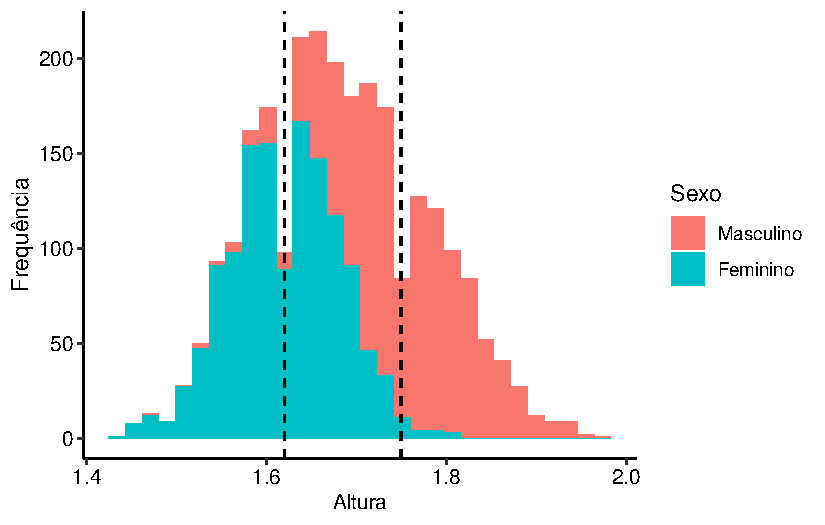
\includegraphics{descritiva_files/figure-pdf/unnamed-chunk-19-1.pdf}

\hypertarget{outras-medidas-de-posiuxe7uxe3o}{%
\subsection{Outras medidas de
posição}\label{outras-medidas-de-posiuxe7uxe3o}}

Também temos outras medidas que representam uma posição de uma
distribuição de valores:

\textbf{Decis}: Divide a distribuição em 10 partes iguais. O 5º decil
representa a mediana.

\textbf{Quartil}: Divide distribuição em quatro partes iguais. O Q2
representa a mediana.

\textbf{Percentil}: Divide a distribuição em 100 partes iguais. O
percentil 50 representa a mediana.

Como todas essas medidas dividem o banco de dados em uma determinada
porcentagem, o termo genérico para elas é quantil e utilizaremos a
função \texttt{quantile()} para calculá-las.

\begin{Shaded}
\begin{Highlighting}[]
\CommentTok{\# Cálculo de exemplo do primeiro decil, primeiro quartil e percentil 99}
\NormalTok{factor\_saq }\SpecialCharTok{|\textgreater{}} 
\NormalTok{  dplyr}\SpecialCharTok{::}\FunctionTok{group\_by}\NormalTok{(sexo) }\SpecialCharTok{|\textgreater{}} 
\NormalTok{  dplyr}\SpecialCharTok{::}\FunctionTok{summarise}\NormalTok{(}\AttributeTok{primeiro\_decil =} \FunctionTok{quantile}\NormalTok{(altura, }\AttributeTok{prob =}\NormalTok{ .}\DecValTok{1}\NormalTok{), }\AttributeTok{primeiro\_quartil =}\FunctionTok{quantile}\NormalTok{(altura, }\AttributeTok{prob =}\NormalTok{ .}\DecValTok{25}\NormalTok{), }\AttributeTok{percentil\_99 =} \FunctionTok{quantile}\NormalTok{(altura, }\AttributeTok{prob =}\NormalTok{ .}\DecValTok{99}\NormalTok{))  }\SpecialCharTok{|\textgreater{}} 
  \CommentTok{\# Reporta os valores na forma de tabela para melhor visualização}
\NormalTok{  knitr}\SpecialCharTok{::}\FunctionTok{kable}\NormalTok{()}
\end{Highlighting}
\end{Shaded}

\begin{longtable}[]{@{}lrrr@{}}
\toprule\noalign{}
sexo & primeiro\_decil & primeiro\_quartil & percentil\_99 \\
\midrule\noalign{}
\endhead
\bottomrule\noalign{}
\endlastfoot
Masculino & 1.66 & 1.70 & 1.92 \\
Feminino & 1.54 & 1.58 & 1.75 \\
\end{longtable}

\hypertarget{medidas-de-dispersuxe3o}{%
\subsection{Medidas de dispersão}\label{medidas-de-dispersuxe3o}}

Medidas de dispersão são valores que indicam o quanto os dados de uma
distribuição estão espalhados ou variam em torno de uma medida central
(como a média).

\textbf{Amplitude}: É a diferença entre o maior e o menor valor de um
conjunto de dados.

\textbf{Variância}: \(\sigma^2 = \frac{\Sigma(xi-\mu)^2}{N}\)

\textbf{Desvio padrão}: \(\sigma = \sqrt{\sigma^2}\)

\textbf{Distância interquartil}: \(DIQ = Q3 - Q1\)

\begin{Shaded}
\begin{Highlighting}[]
\CommentTok{\# Vamos calcular as métricas acima para o nosso a altura dos indivíduos em nosso banco de dados}

\NormalTok{factor\_saq }\SpecialCharTok{|\textgreater{}} 
\NormalTok{  dplyr}\SpecialCharTok{::}\FunctionTok{group\_by}\NormalTok{(sexo) }\SpecialCharTok{|\textgreater{}} 
\NormalTok{  dplyr}\SpecialCharTok{::}\FunctionTok{summarise}\NormalTok{(}\AttributeTok{variancia =} \FunctionTok{var}\NormalTok{(altura), }\AttributeTok{desvio\_padrao =} \FunctionTok{sd}\NormalTok{(altura), }\AttributeTok{amplitude =} \FunctionTok{max}\NormalTok{(altura) }\SpecialCharTok{{-}} \FunctionTok{min}\NormalTok{(altura), }\AttributeTok{distancia\_interquartil =} \FunctionTok{IQR}\NormalTok{(altura))  }\SpecialCharTok{|\textgreater{}} 
  \CommentTok{\# Reporta os valores na forma de tabela para melhor visualização}
\NormalTok{  knitr}\SpecialCharTok{::}\FunctionTok{kable}\NormalTok{()}
\end{Highlighting}
\end{Shaded}

\begin{longtable}[]{@{}
  >{\raggedright\arraybackslash}p{(\columnwidth - 8\tabcolsep) * \real{0.1493}}
  >{\raggedleft\arraybackslash}p{(\columnwidth - 8\tabcolsep) * \real{0.1493}}
  >{\raggedleft\arraybackslash}p{(\columnwidth - 8\tabcolsep) * \real{0.2090}}
  >{\raggedleft\arraybackslash}p{(\columnwidth - 8\tabcolsep) * \real{0.1493}}
  >{\raggedleft\arraybackslash}p{(\columnwidth - 8\tabcolsep) * \real{0.3433}}@{}}
\toprule\noalign{}
\begin{minipage}[b]{\linewidth}\raggedright
sexo
\end{minipage} & \begin{minipage}[b]{\linewidth}\raggedleft
variancia
\end{minipage} & \begin{minipage}[b]{\linewidth}\raggedleft
desvio\_padrao
\end{minipage} & \begin{minipage}[b]{\linewidth}\raggedleft
amplitude
\end{minipage} & \begin{minipage}[b]{\linewidth}\raggedleft
distancia\_interquartil
\end{minipage} \\
\midrule\noalign{}
\endhead
\bottomrule\noalign{}
\endlastfoot
Masculino & 0.0053669 & 0.0732594 & 0.50 & 0.10 \\
Feminino & 0.0037084 & 0.0608964 & 0.37 & 0.08 \\
\end{longtable}

O gráfico de densidade permite uma boa visualização da dispersão dos
dados.

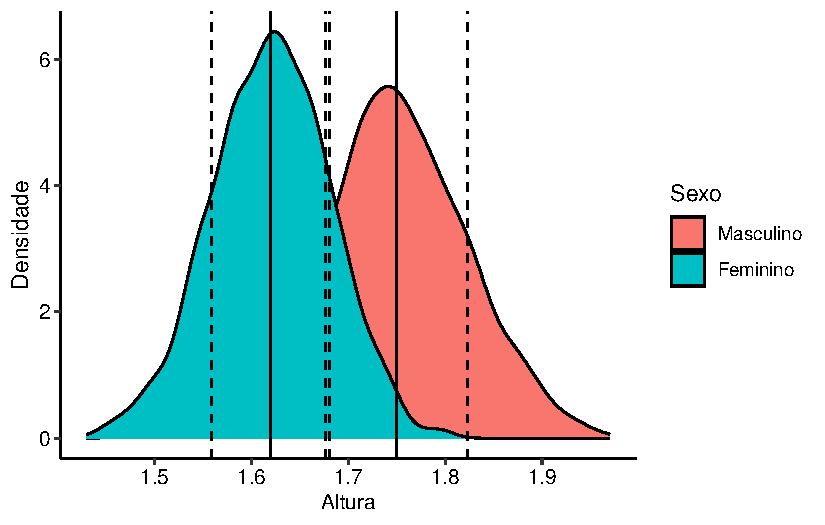
\includegraphics{descritiva_files/figure-pdf/unnamed-chunk-23-1.pdf}

\hypertarget{descrevendo-variuxe1veis-categuxf3ricas}{%
\section{Descrevendo variáveis
categóricas}\label{descrevendo-variuxe1veis-categuxf3ricas}}

\hypertarget{tabela-de-continguxeancia-e-gruxe1fico-em-barras}{%
\subsection{Tabela de contingência e gráfico em
barras}\label{tabela-de-continguxeancia-e-gruxe1fico-em-barras}}

Para variáveis categóricas, costuma-se trabalhar com a frequência de
cada categoria. Uma boa forma de descrevê-las é pela tabela de
contingência:

\begin{Shaded}
\begin{Highlighting}[]
\CommentTok{\# Cria tabela de contingência para a variável raca\_etnia}
\NormalTok{factor\_saq }\SpecialCharTok{|\textgreater{}} 
\NormalTok{  dplyr}\SpecialCharTok{::}\FunctionTok{group\_by}\NormalTok{(sexo) }\SpecialCharTok{|\textgreater{}} 
\NormalTok{  dplyr}\SpecialCharTok{::}\FunctionTok{pull}\NormalTok{(raca\_etnia) }\SpecialCharTok{|\textgreater{}} 
\NormalTok{  base}\SpecialCharTok{::}\FunctionTok{table}\NormalTok{() }\SpecialCharTok{|\textgreater{}} 
\NormalTok{  knitr}\SpecialCharTok{::}\FunctionTok{kable}\NormalTok{(}\AttributeTok{col.names =} \FunctionTok{c}\NormalTok{(}\StringTok{"Raça/Etnia"}\NormalTok{, }\StringTok{"Frequência"}\NormalTok{))}
\end{Highlighting}
\end{Shaded}

\begin{longtable}[]{@{}lr@{}}
\toprule\noalign{}
Raça/Etnia & Frequência \\
\midrule\noalign{}
\endhead
\bottomrule\noalign{}
\endlastfoot
Branca & 1096 \\
Preta & 258 \\
Parda & 1217 \\
\end{longtable}

Também podemos utilizar um gráfico de barras\footnote{Apesar de
  parecidos, o gráfico de barras é um tipo de representação distinta do
  histograma. Enquanto o último é utilizado para representar dados
  numéricos, o gráfico de barras representa a frequência de dados
  categóricos.} para representar a frequência de cada categoria. Veja o
exemplo abaixo, que mostra a quantidade de pessoas em cada categoria de
Raça/Etnia, por sexo.

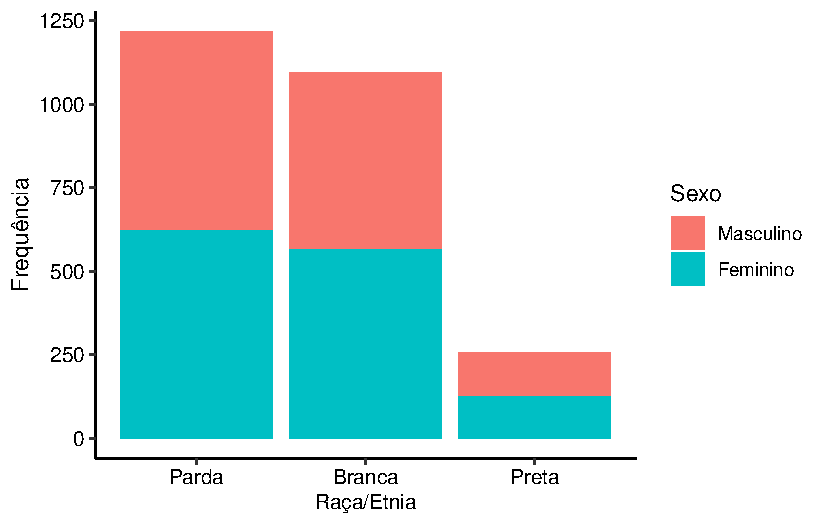
\includegraphics{descritiva_files/figure-pdf/unnamed-chunk-25-1.pdf}

Quando pensamos nas respostas do questinário RAQ-23, poderíamos
analisá-lo em forma de gráfico de barras, como fizemos com a variável
Raça/Etnia:

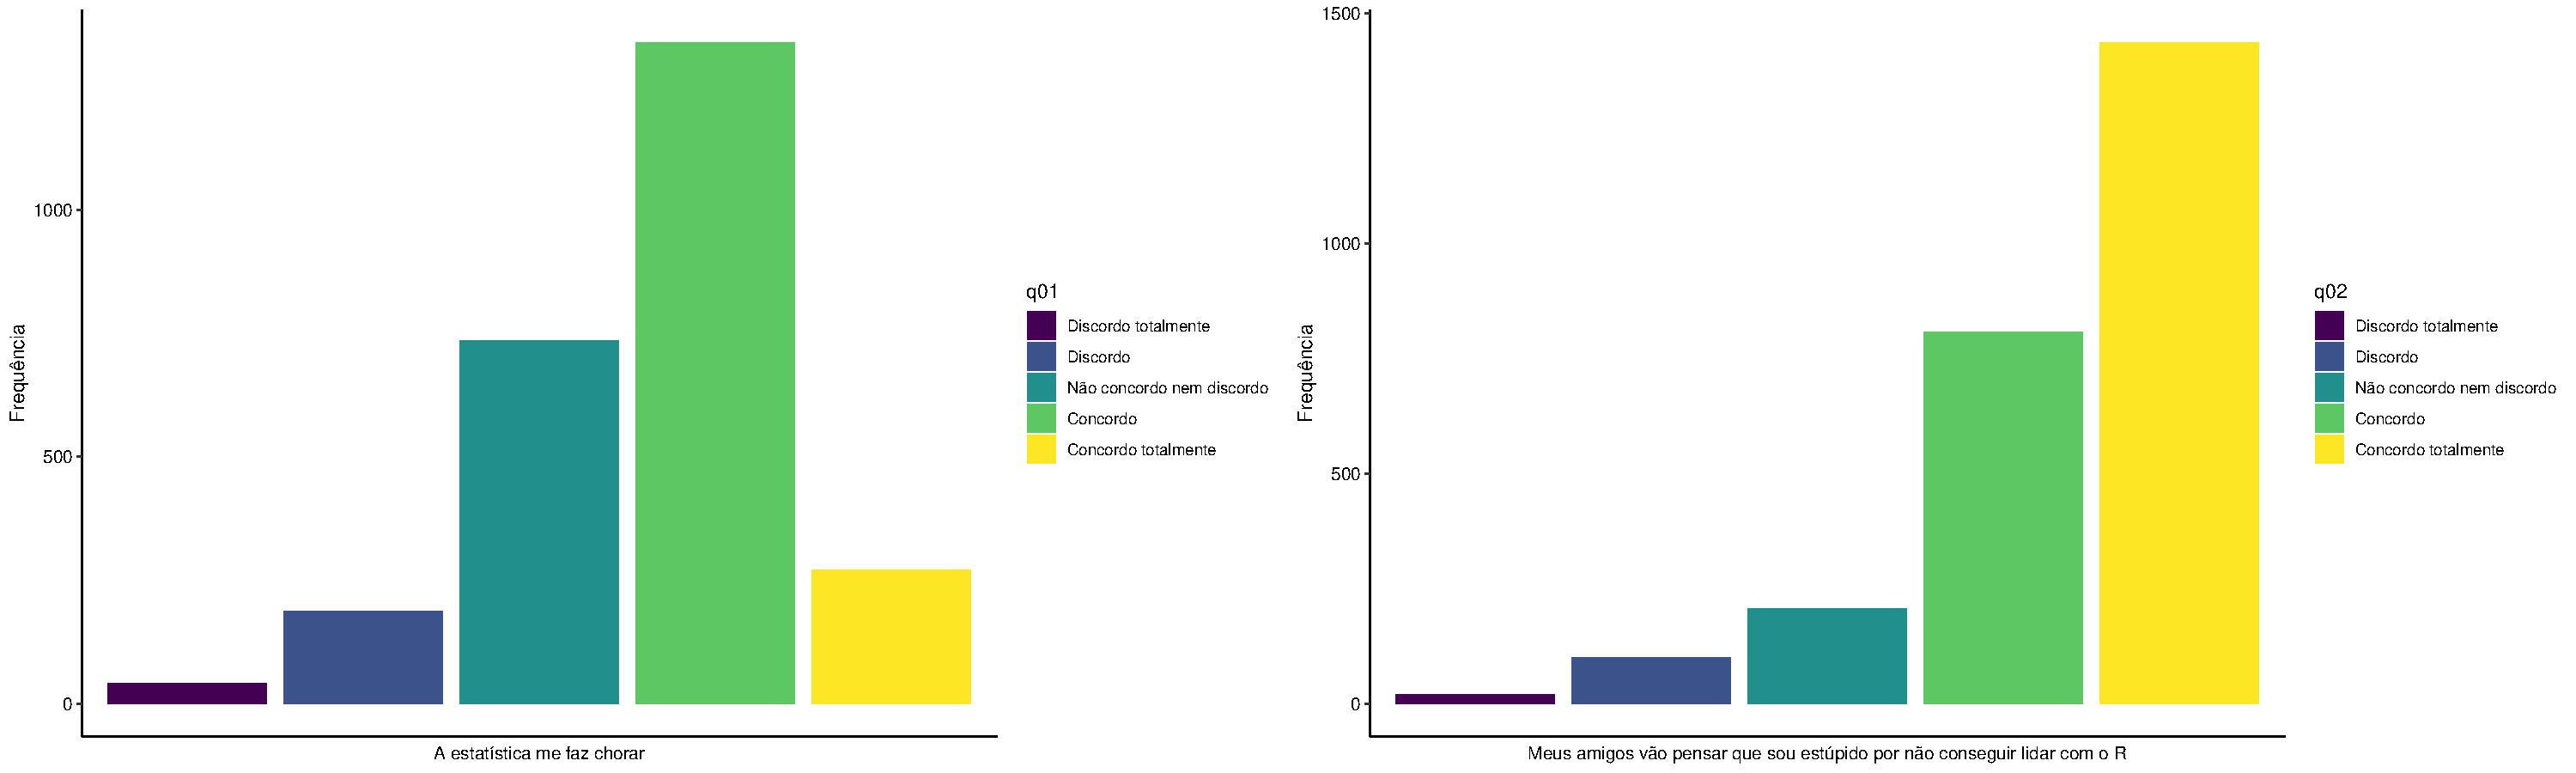
\includegraphics{descritiva_files/figure-pdf/unnamed-chunk-26-1.pdf}

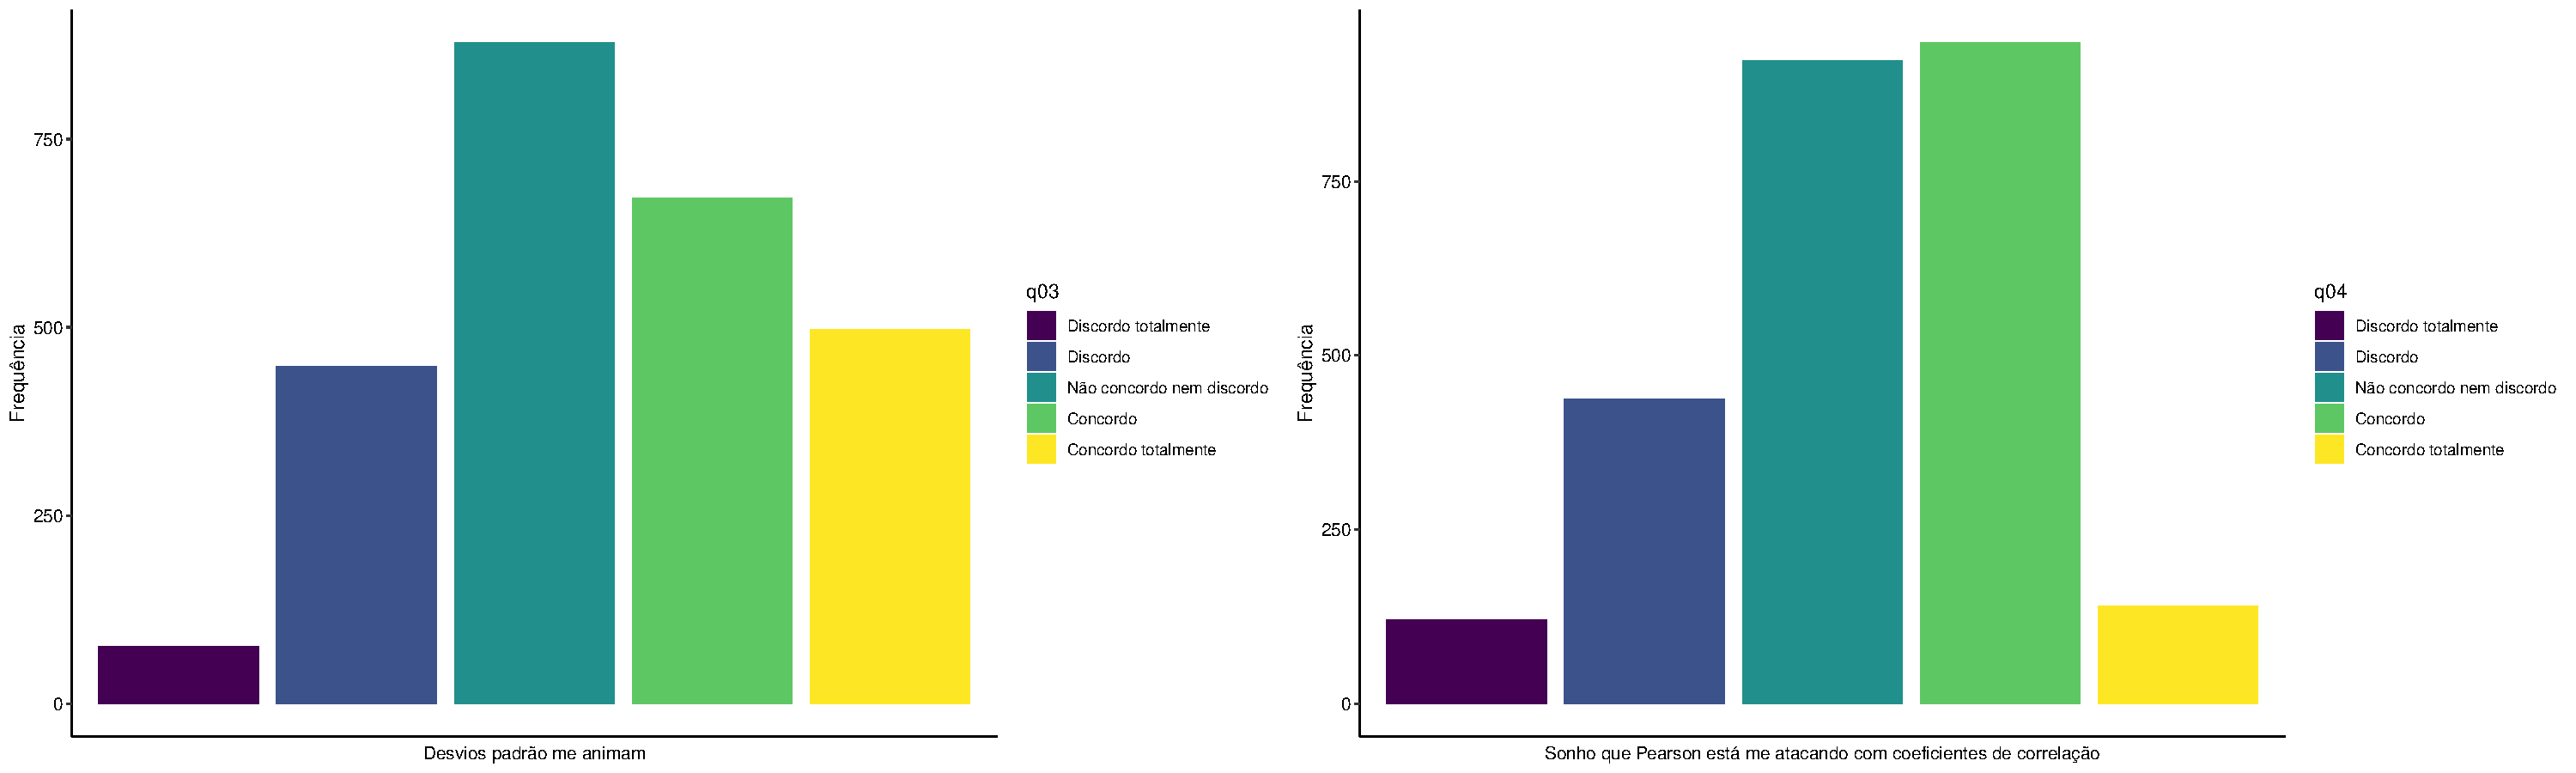
\includegraphics{descritiva_files/figure-pdf/unnamed-chunk-26-2.pdf}

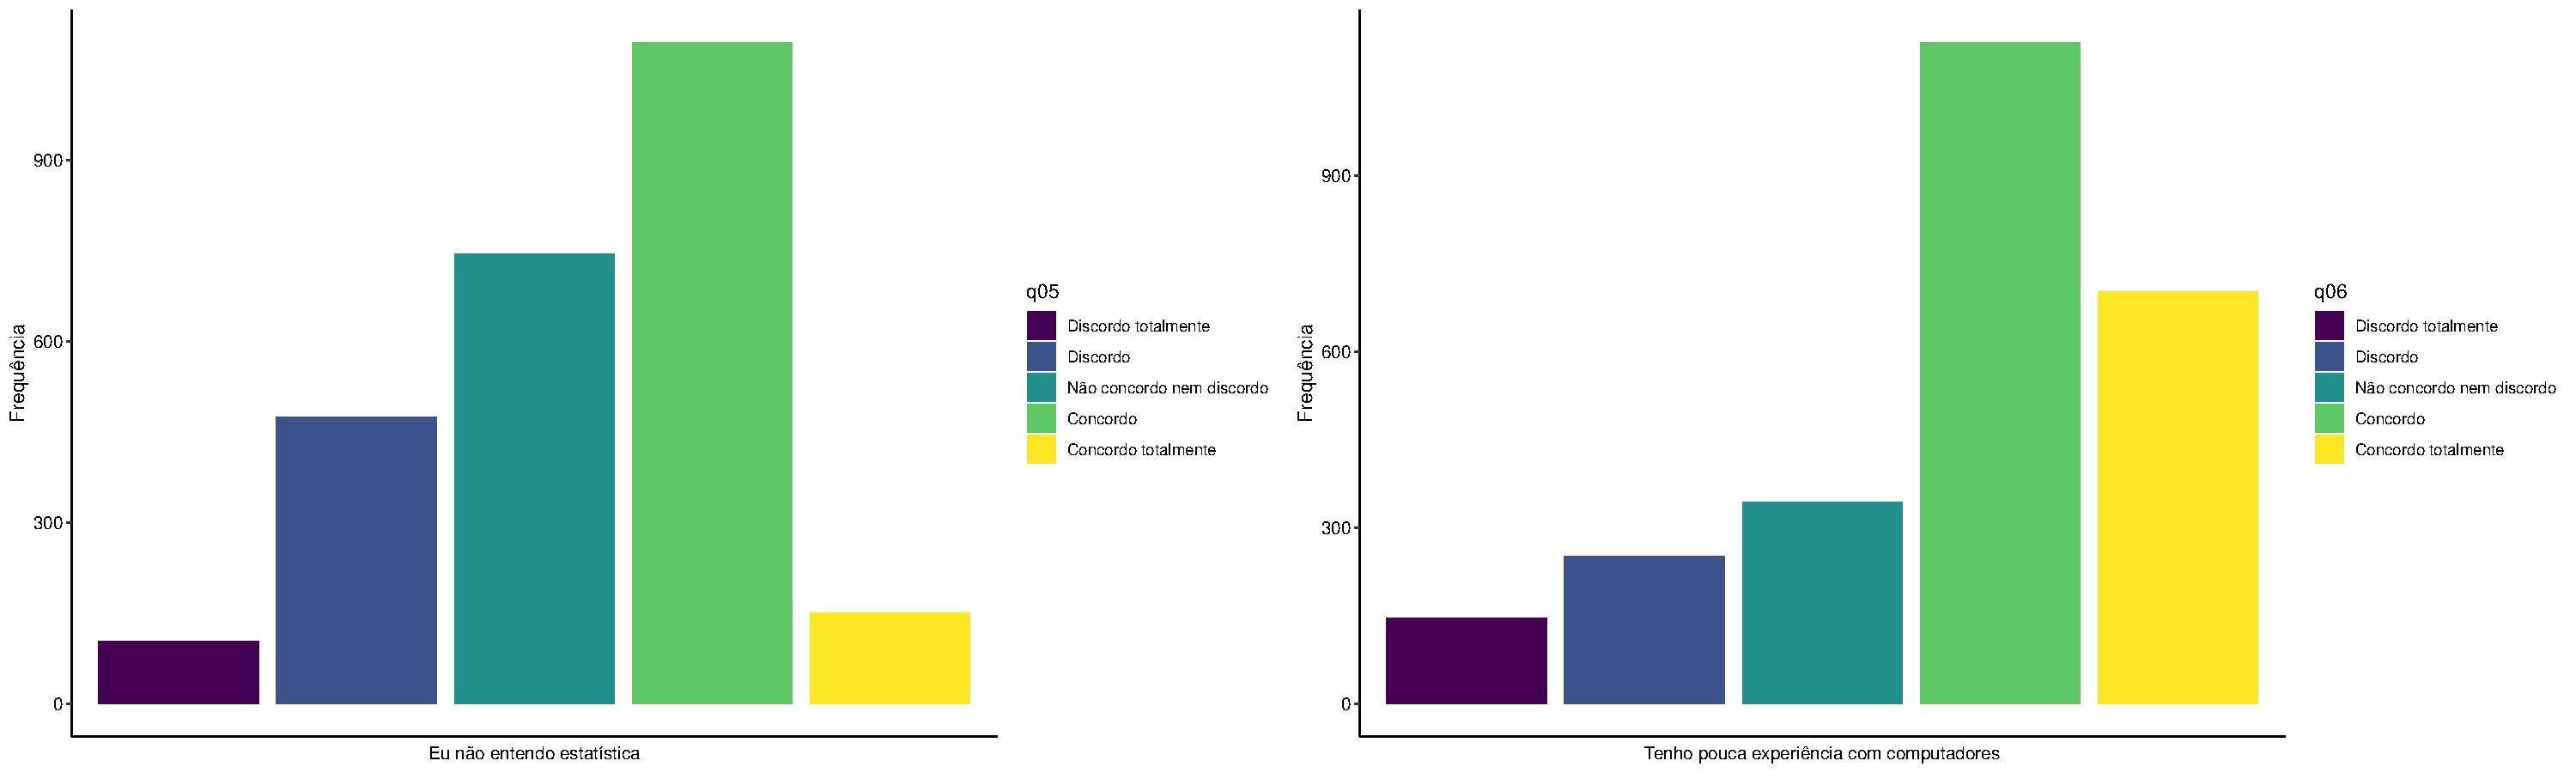
\includegraphics{descritiva_files/figure-pdf/unnamed-chunk-26-3.pdf}

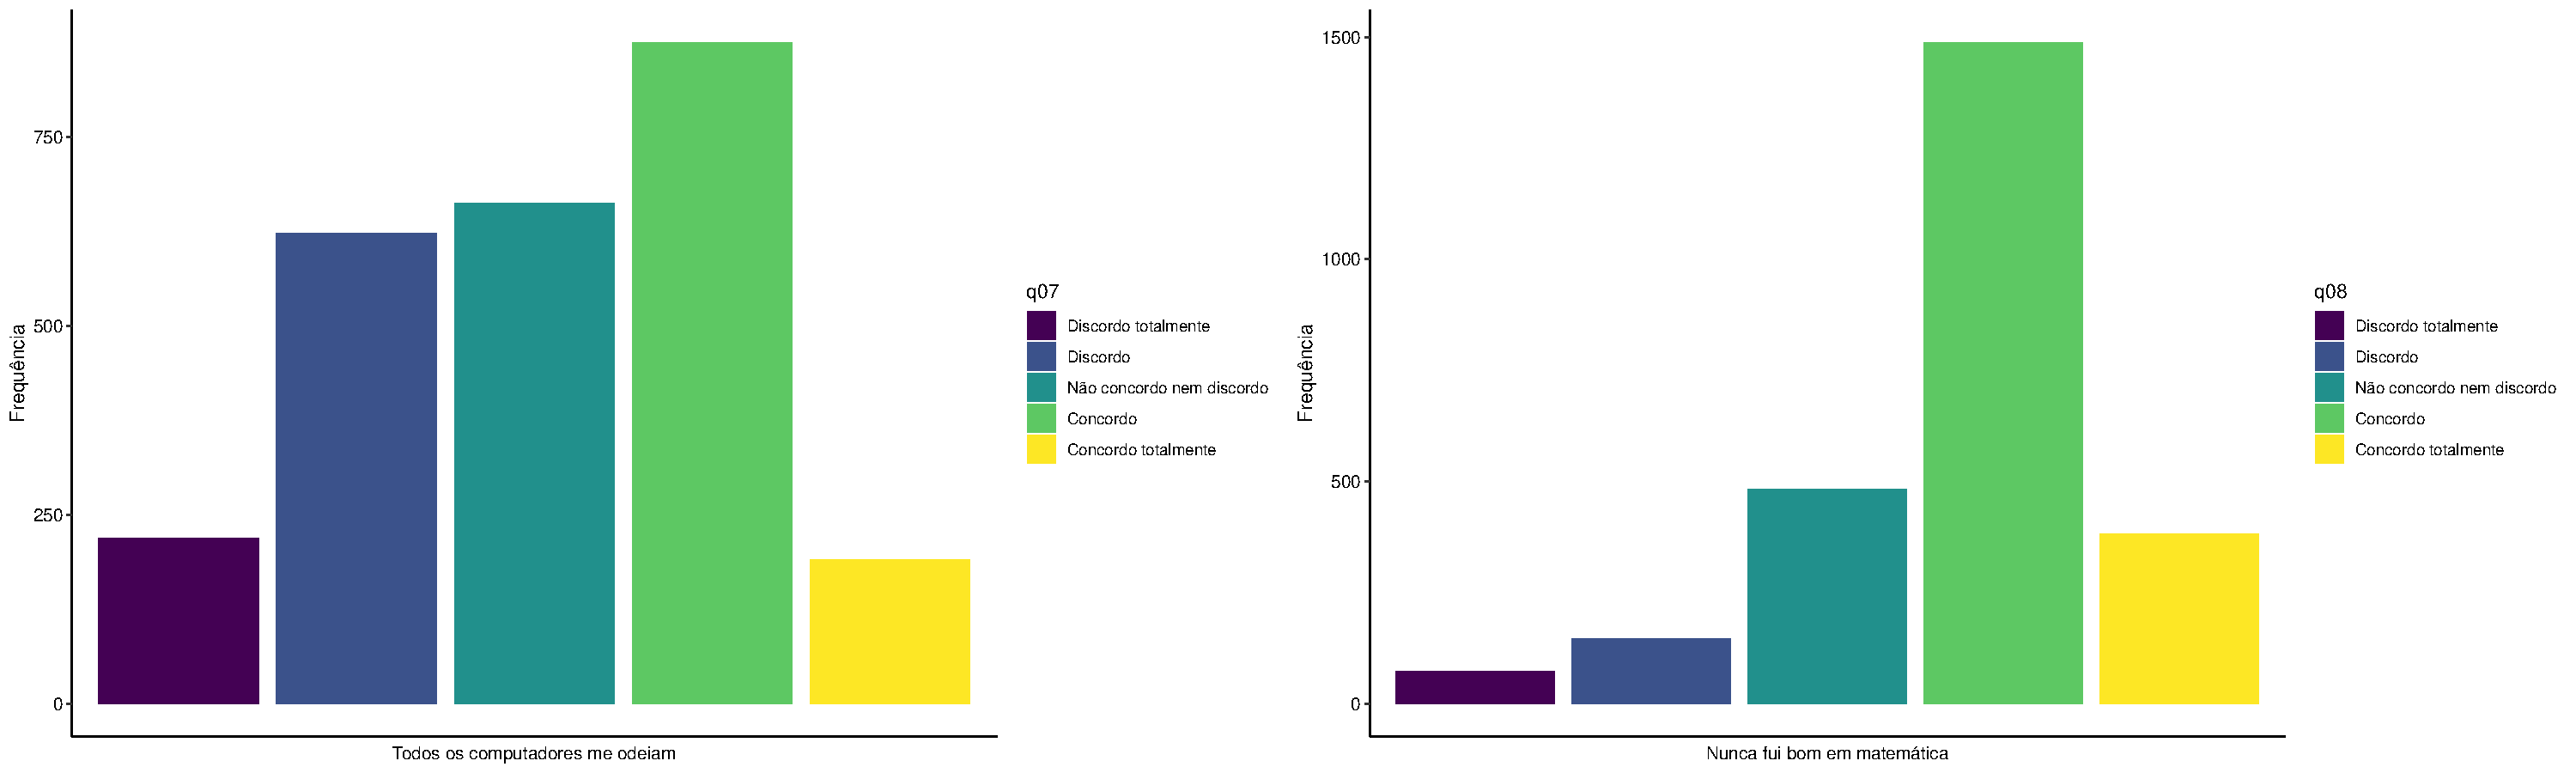
\includegraphics{descritiva_files/figure-pdf/unnamed-chunk-26-4.pdf}

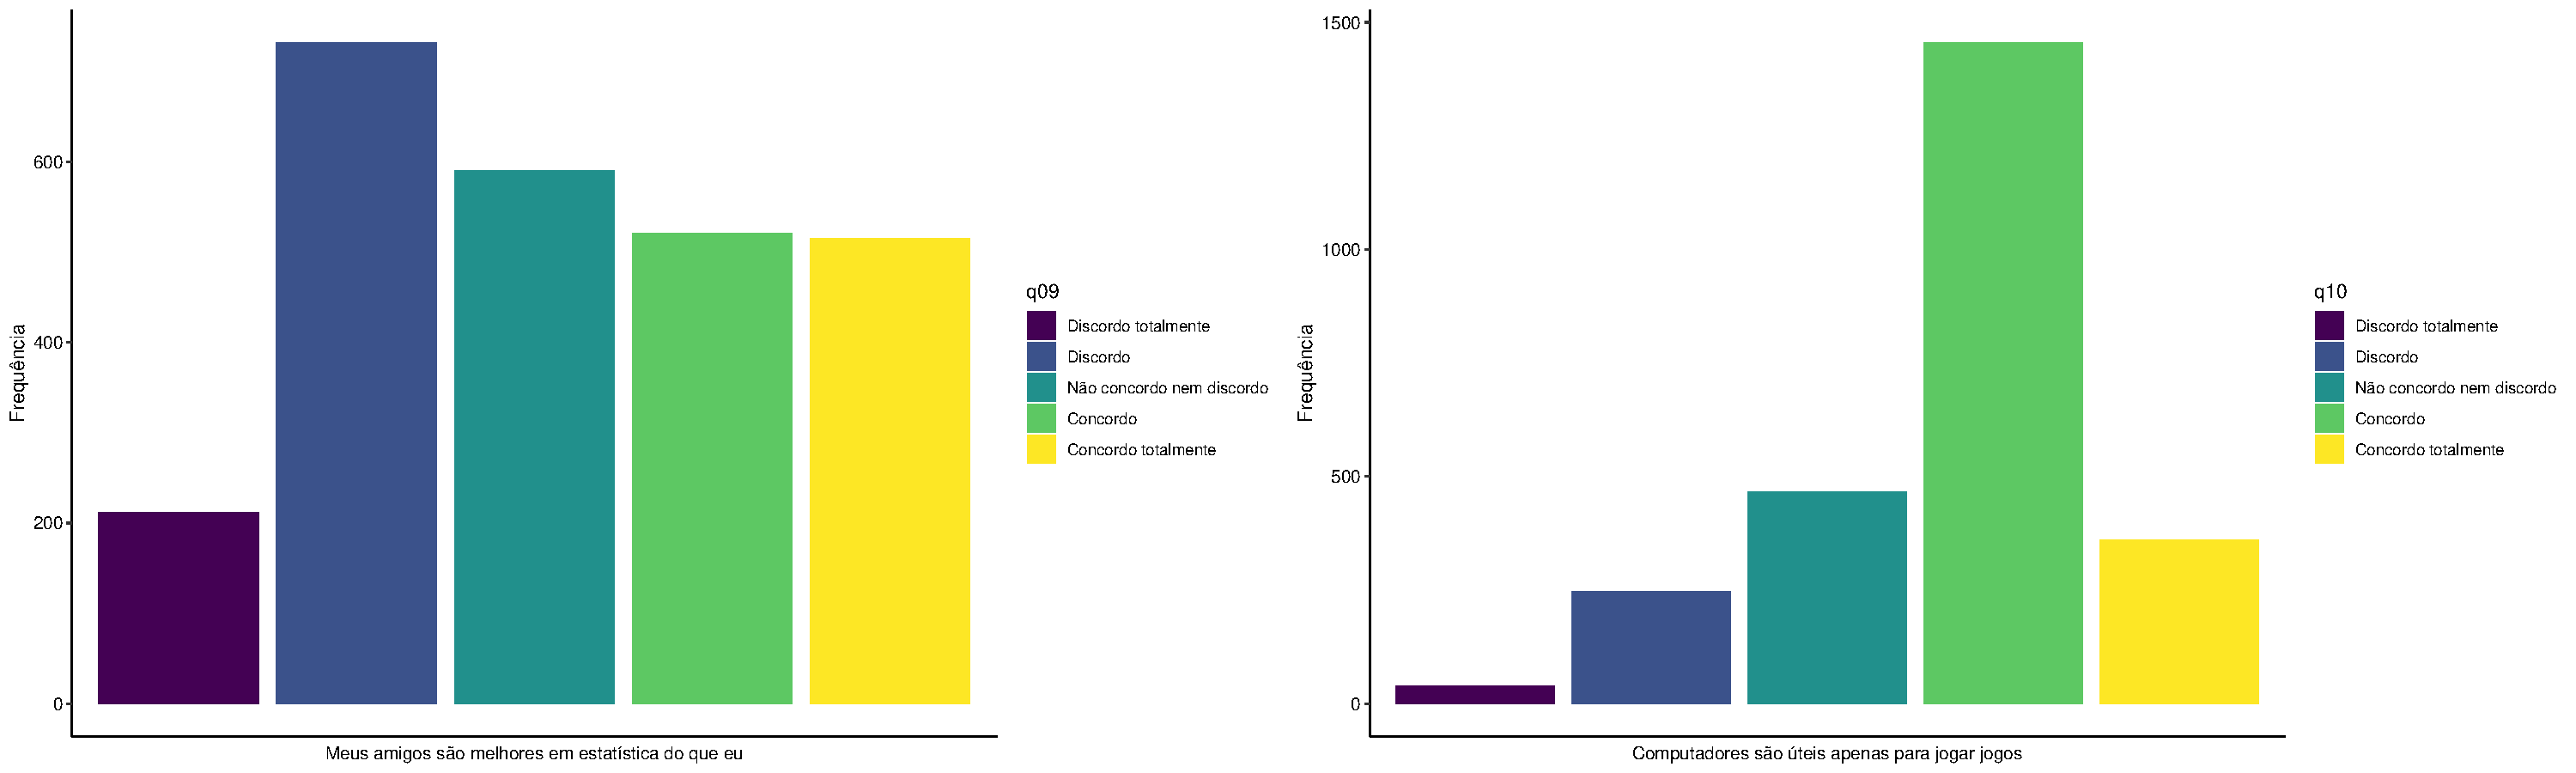
\includegraphics{descritiva_files/figure-pdf/unnamed-chunk-26-5.pdf}

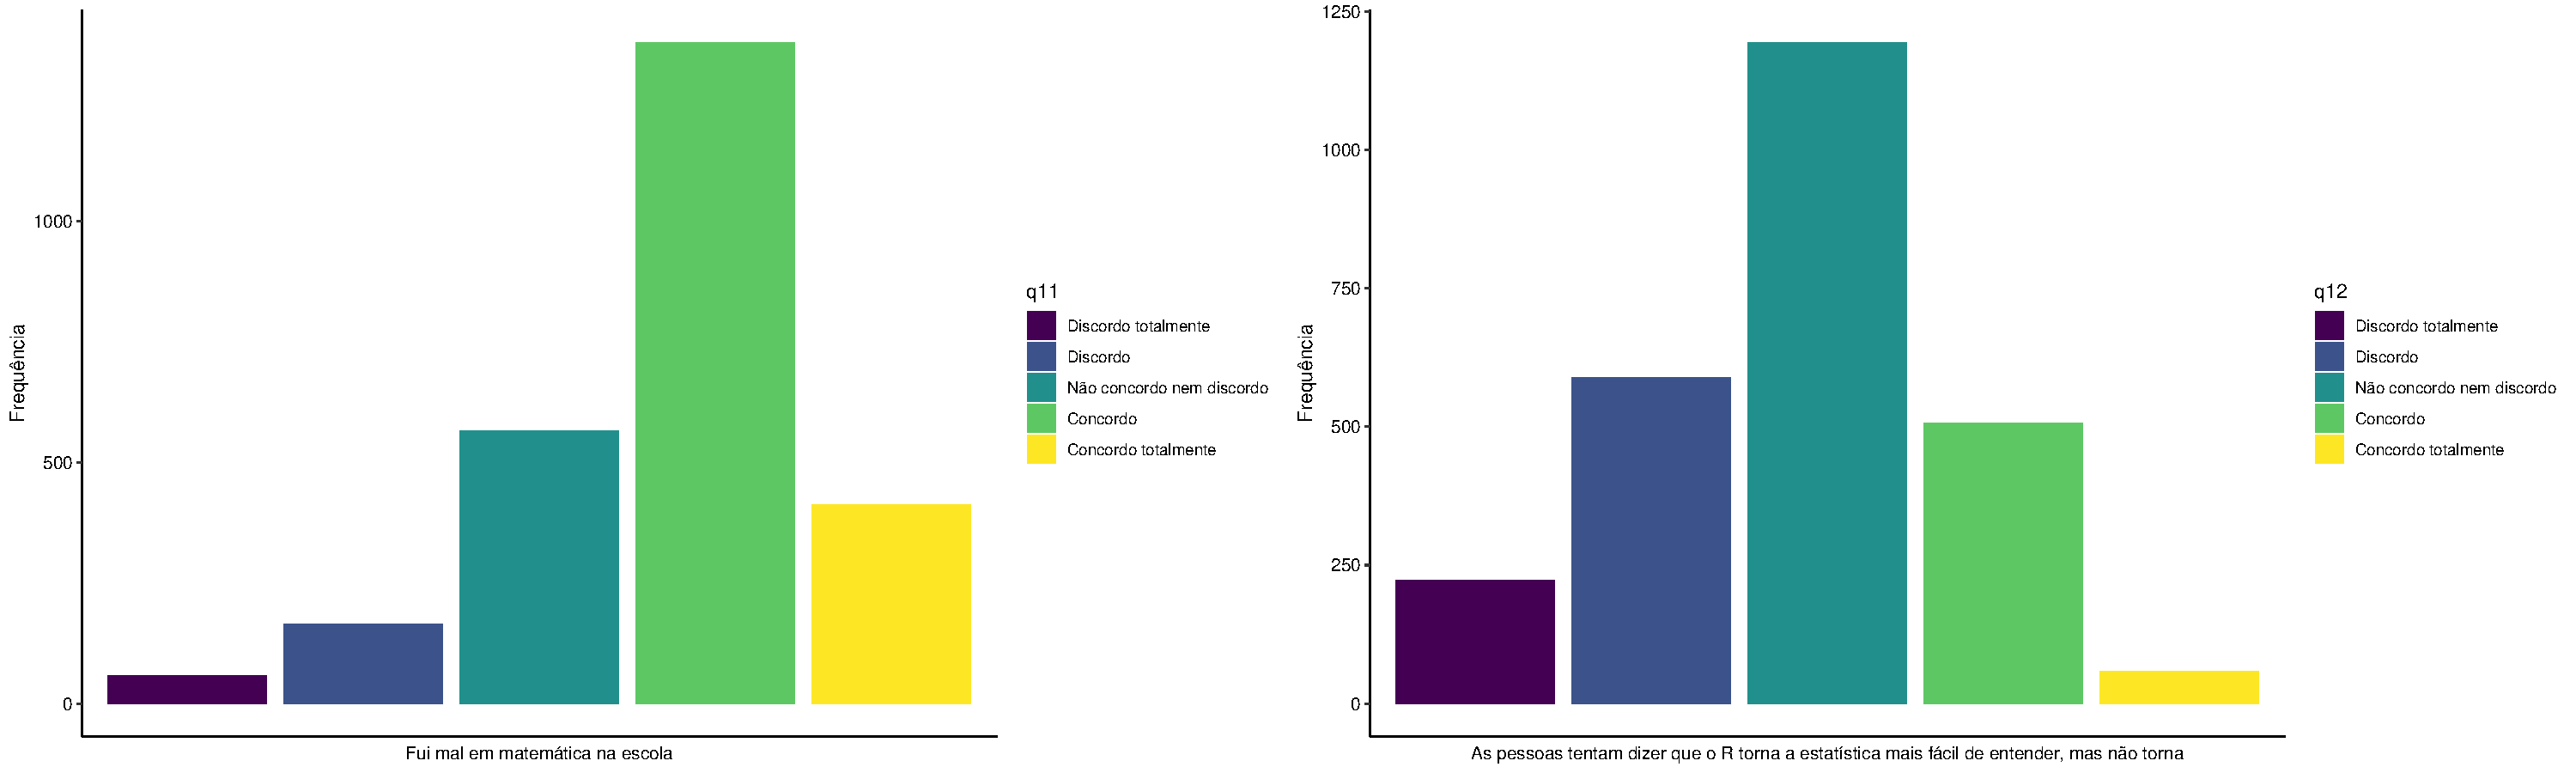
\includegraphics{descritiva_files/figure-pdf/unnamed-chunk-26-6.pdf}

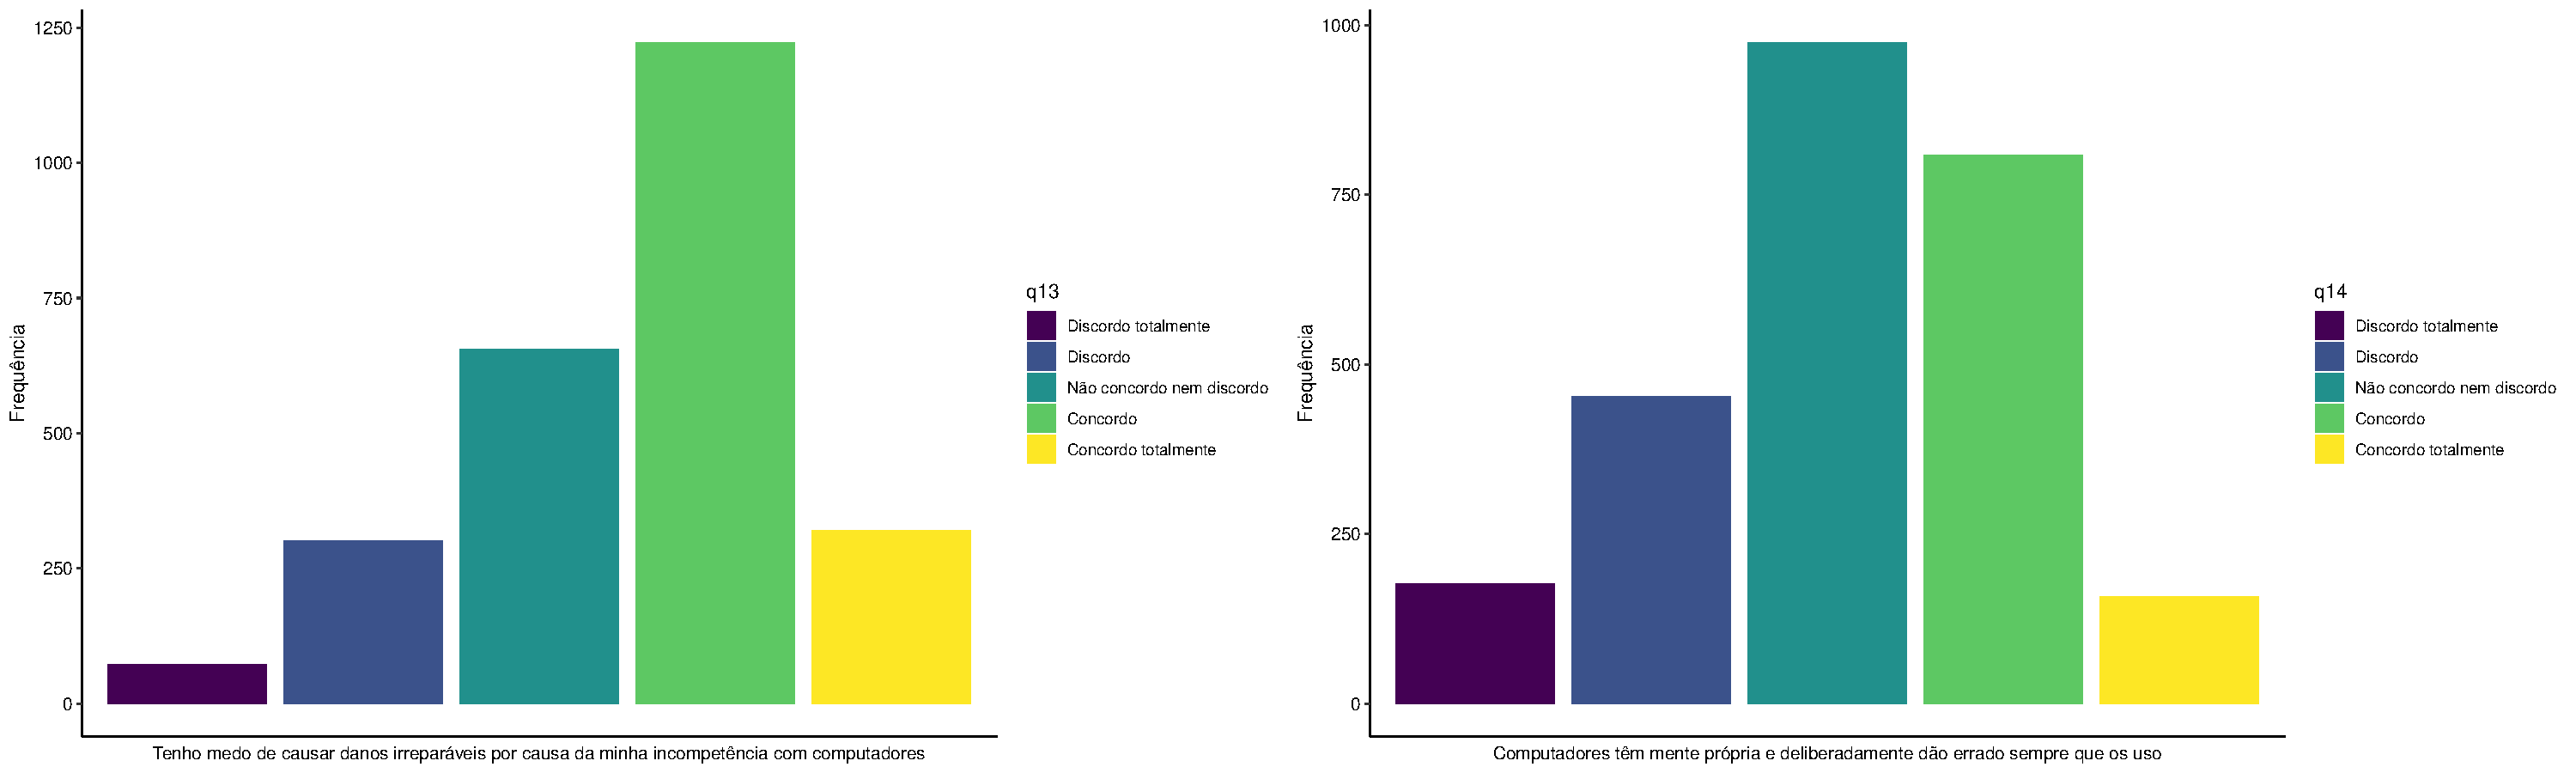
\includegraphics{descritiva_files/figure-pdf/unnamed-chunk-26-7.pdf}

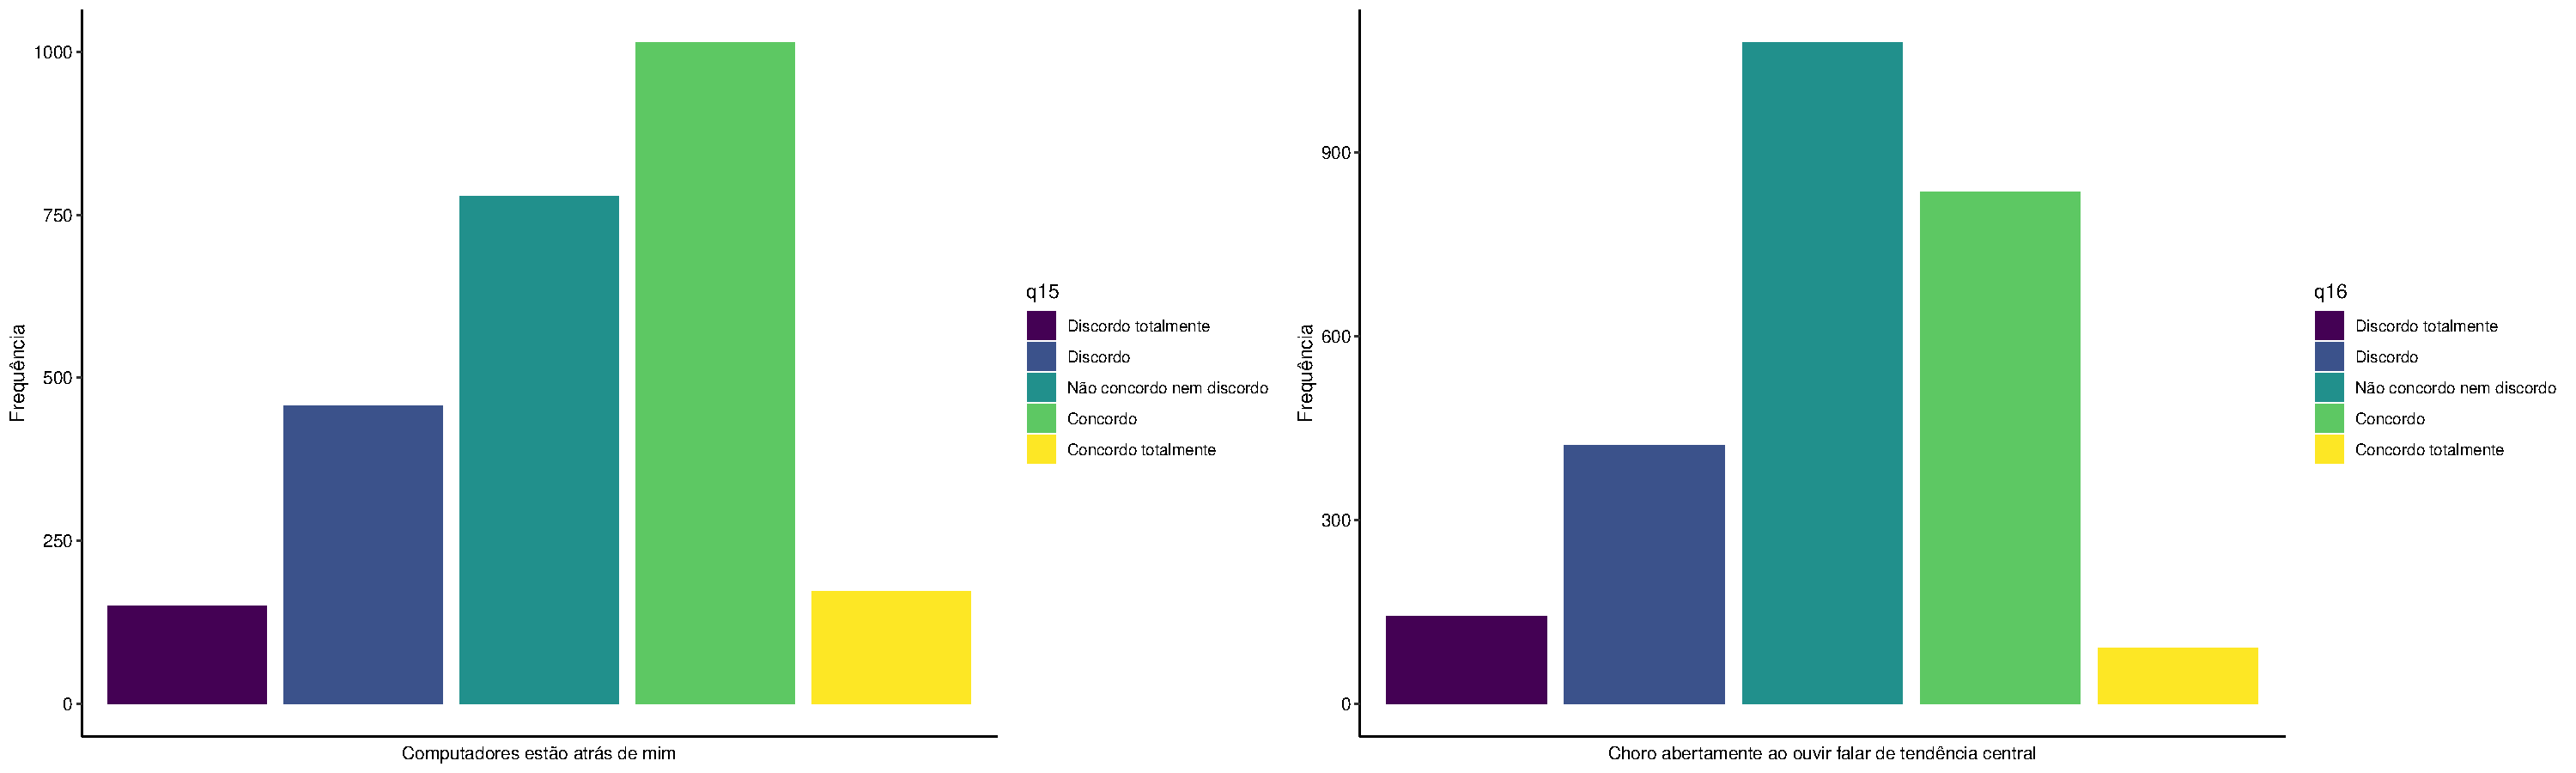
\includegraphics{descritiva_files/figure-pdf/unnamed-chunk-26-8.pdf}

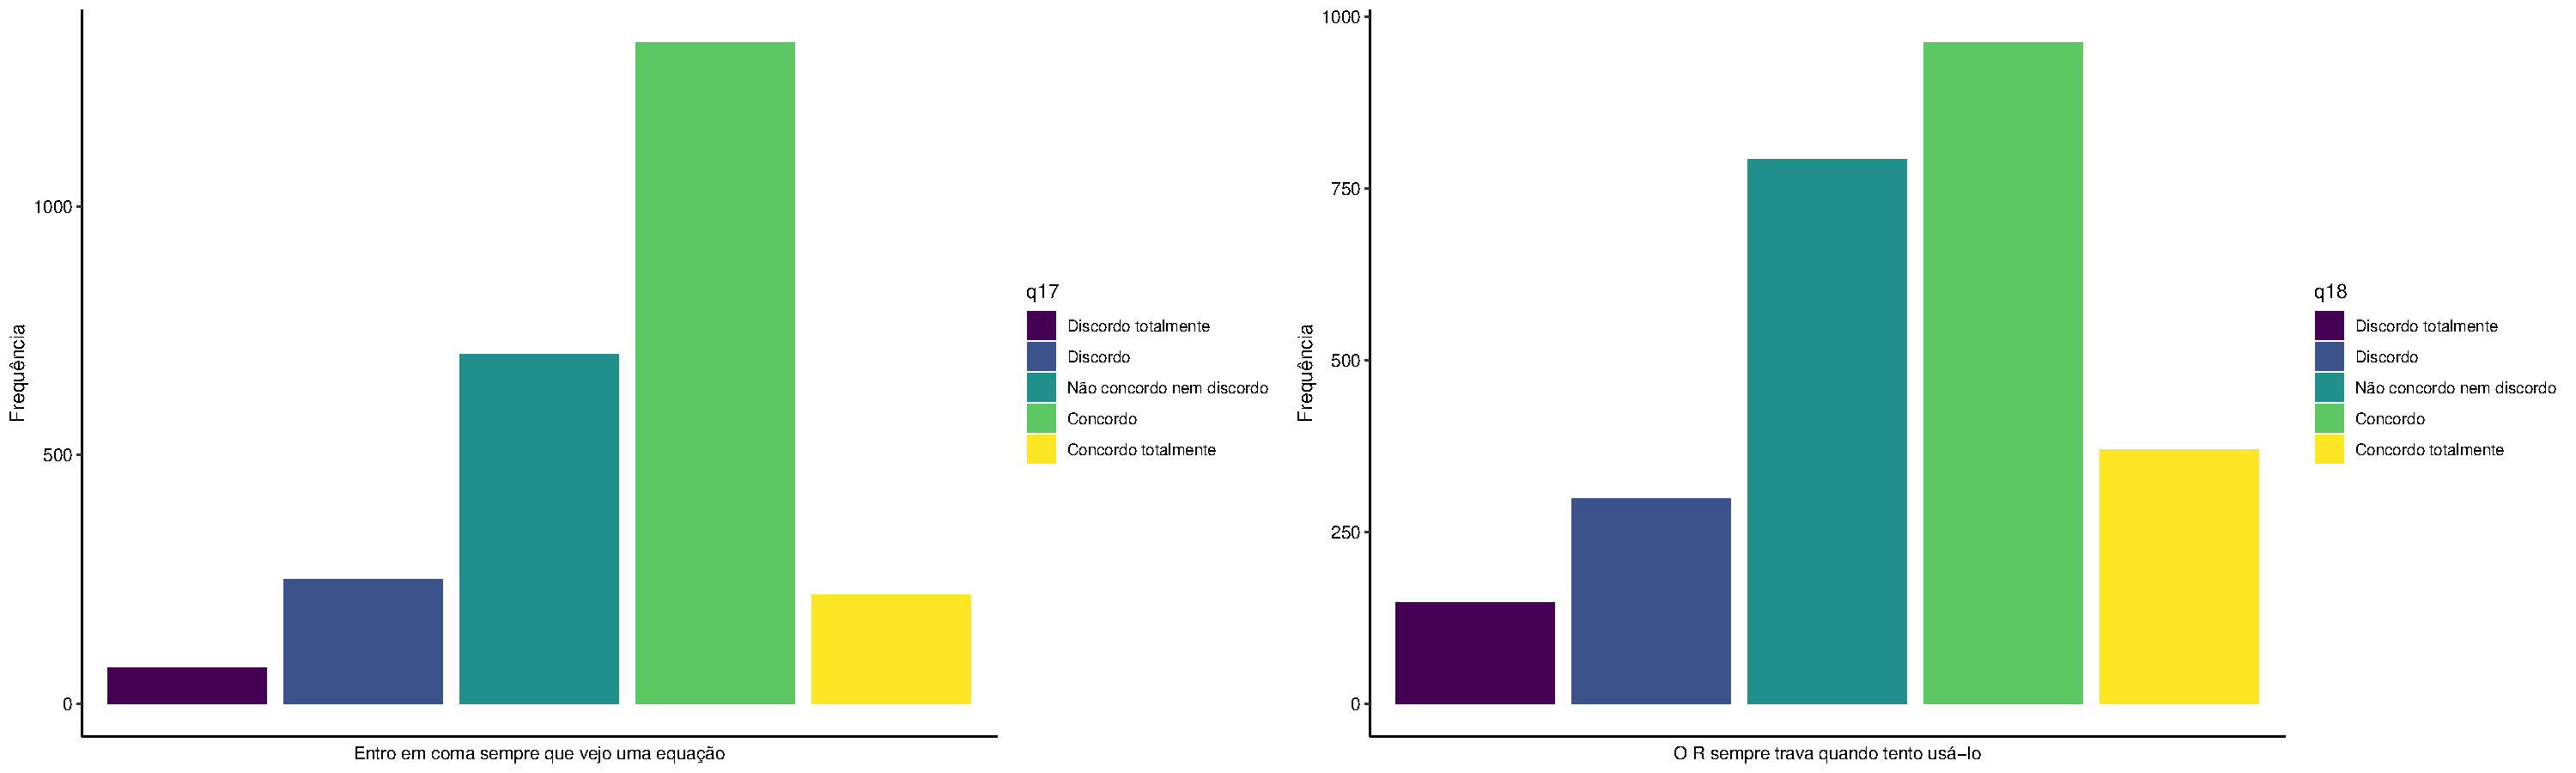
\includegraphics{descritiva_files/figure-pdf/unnamed-chunk-26-9.pdf}

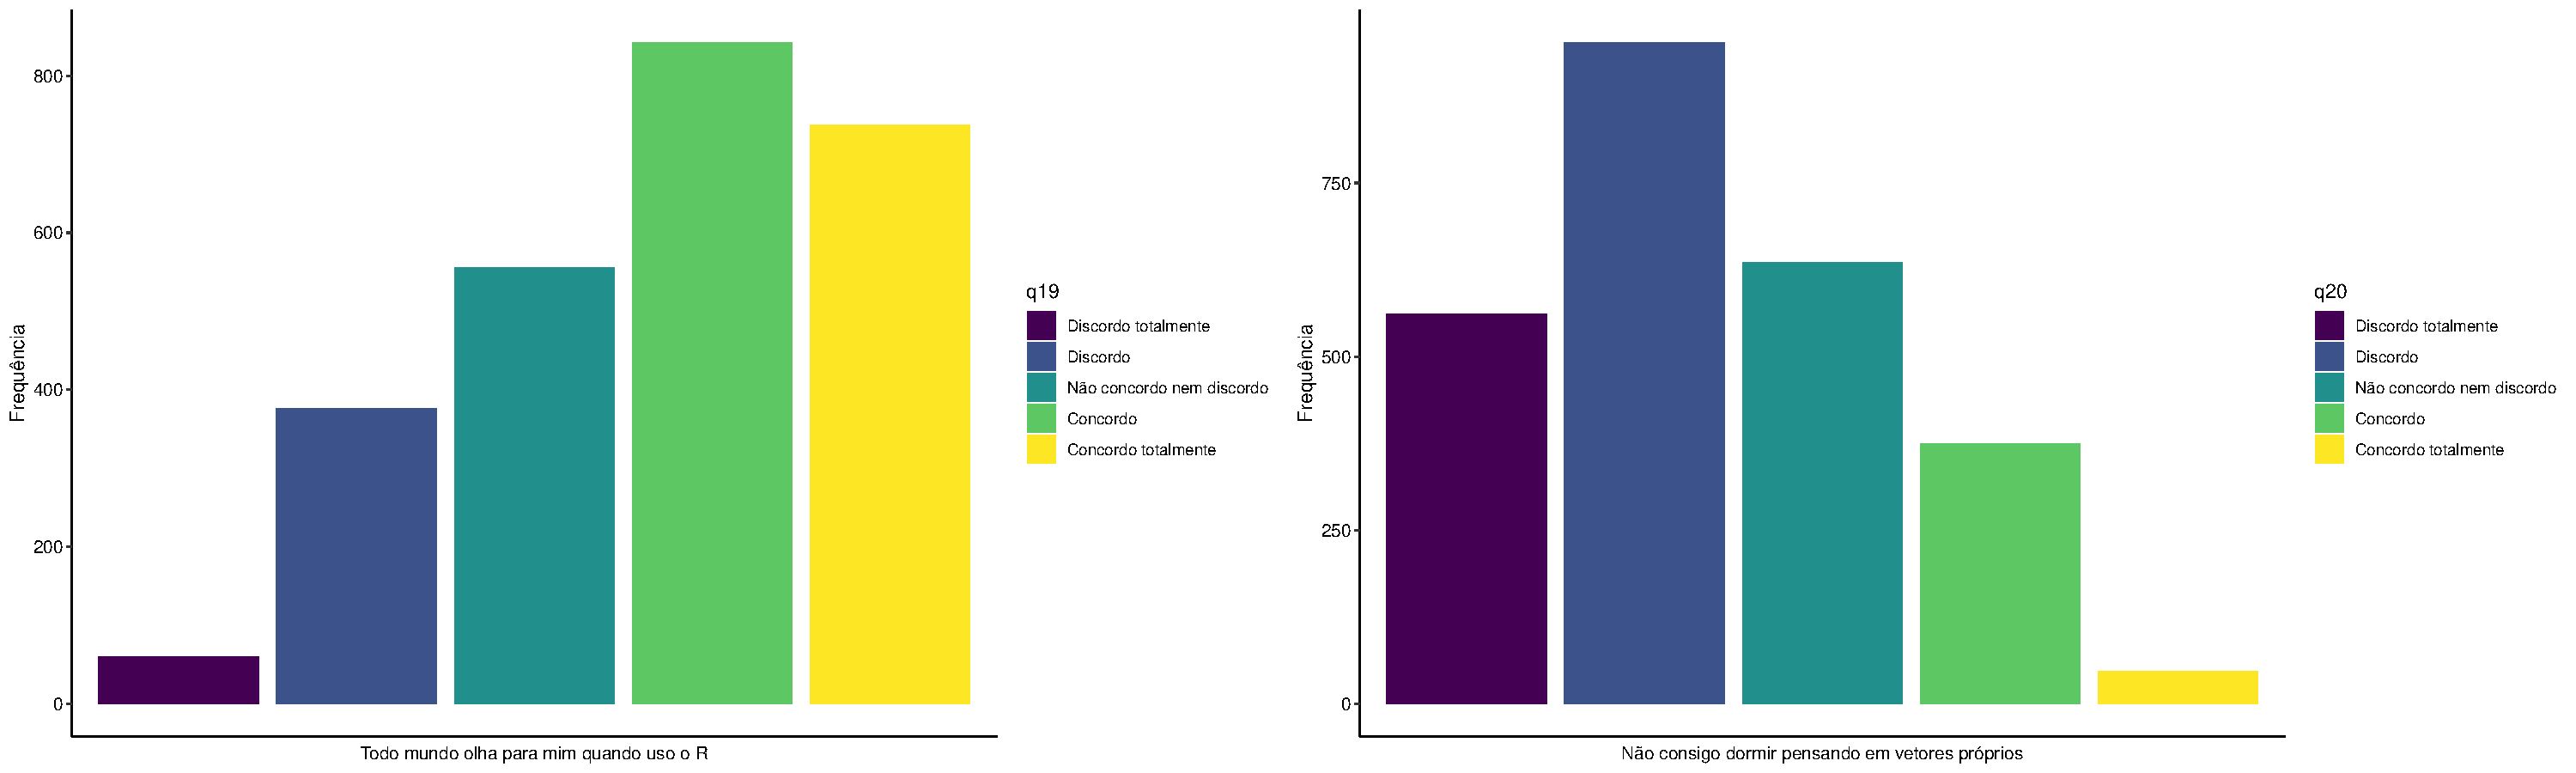
\includegraphics{descritiva_files/figure-pdf/unnamed-chunk-26-10.pdf}

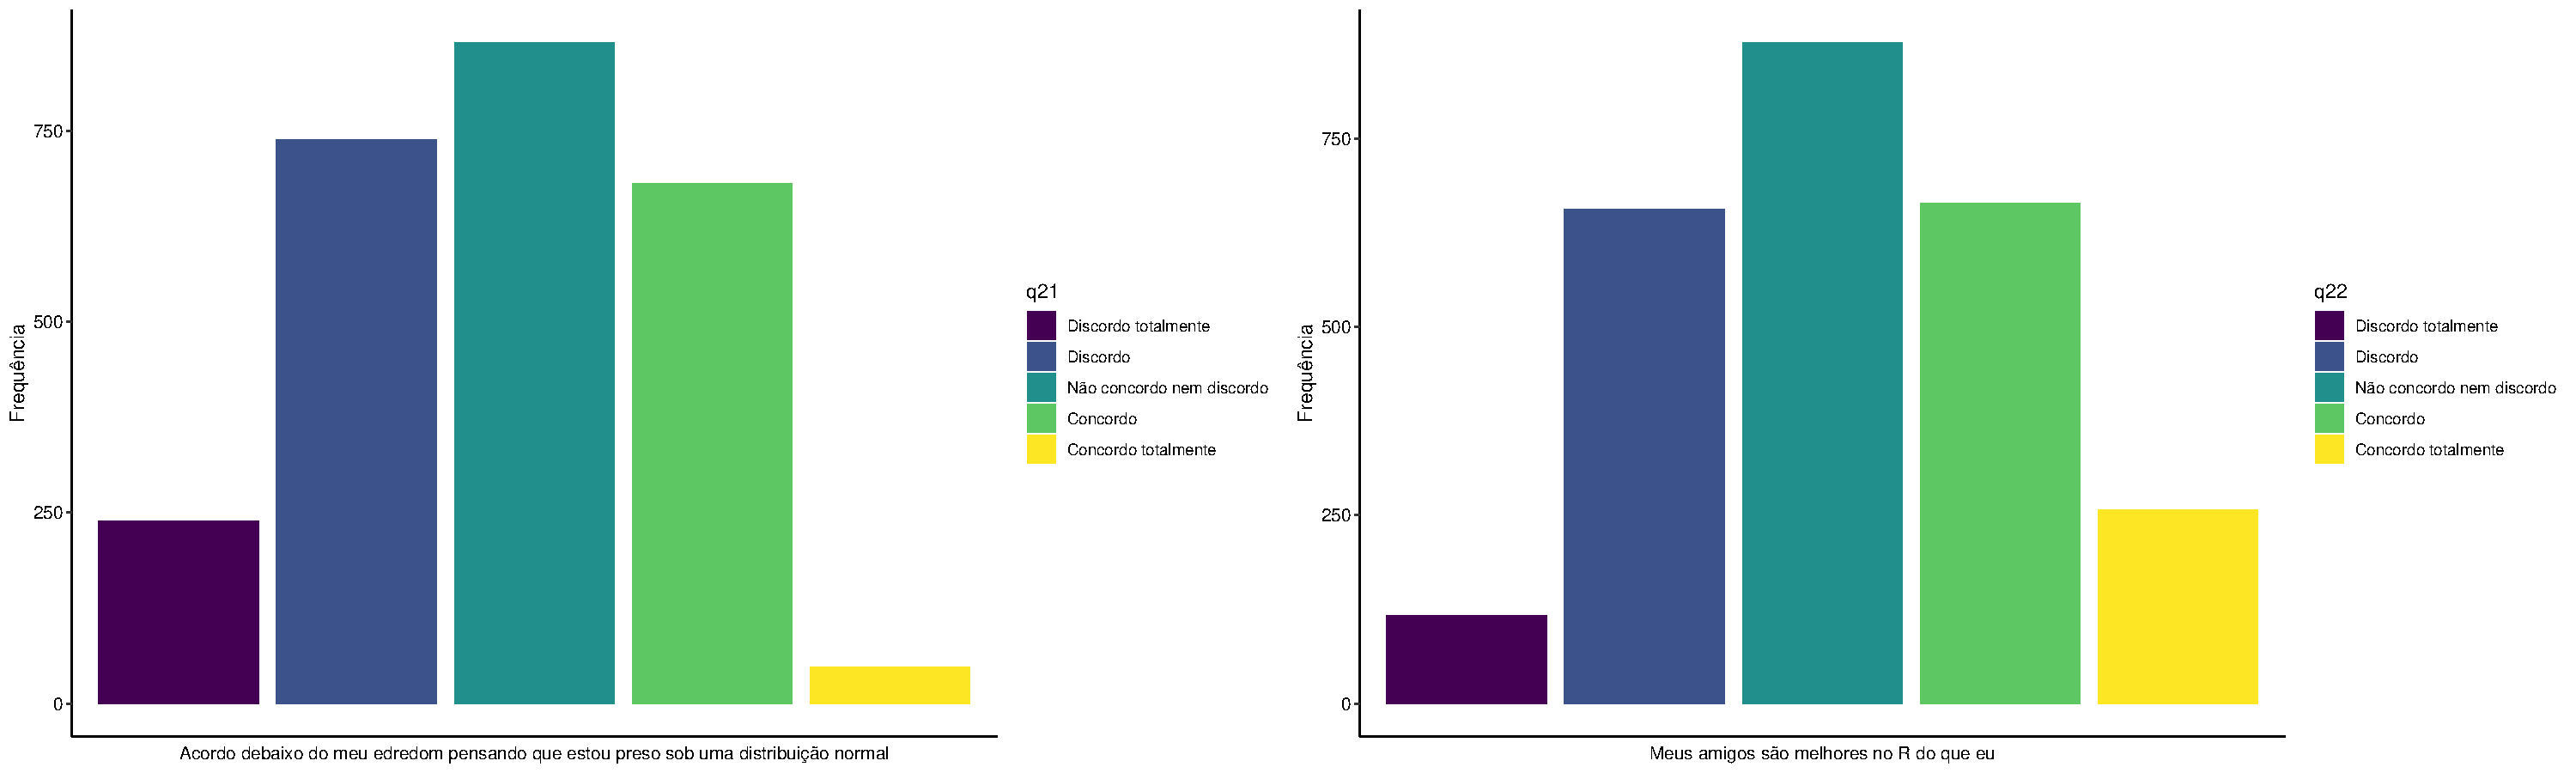
\includegraphics{descritiva_files/figure-pdf/unnamed-chunk-26-11.pdf}

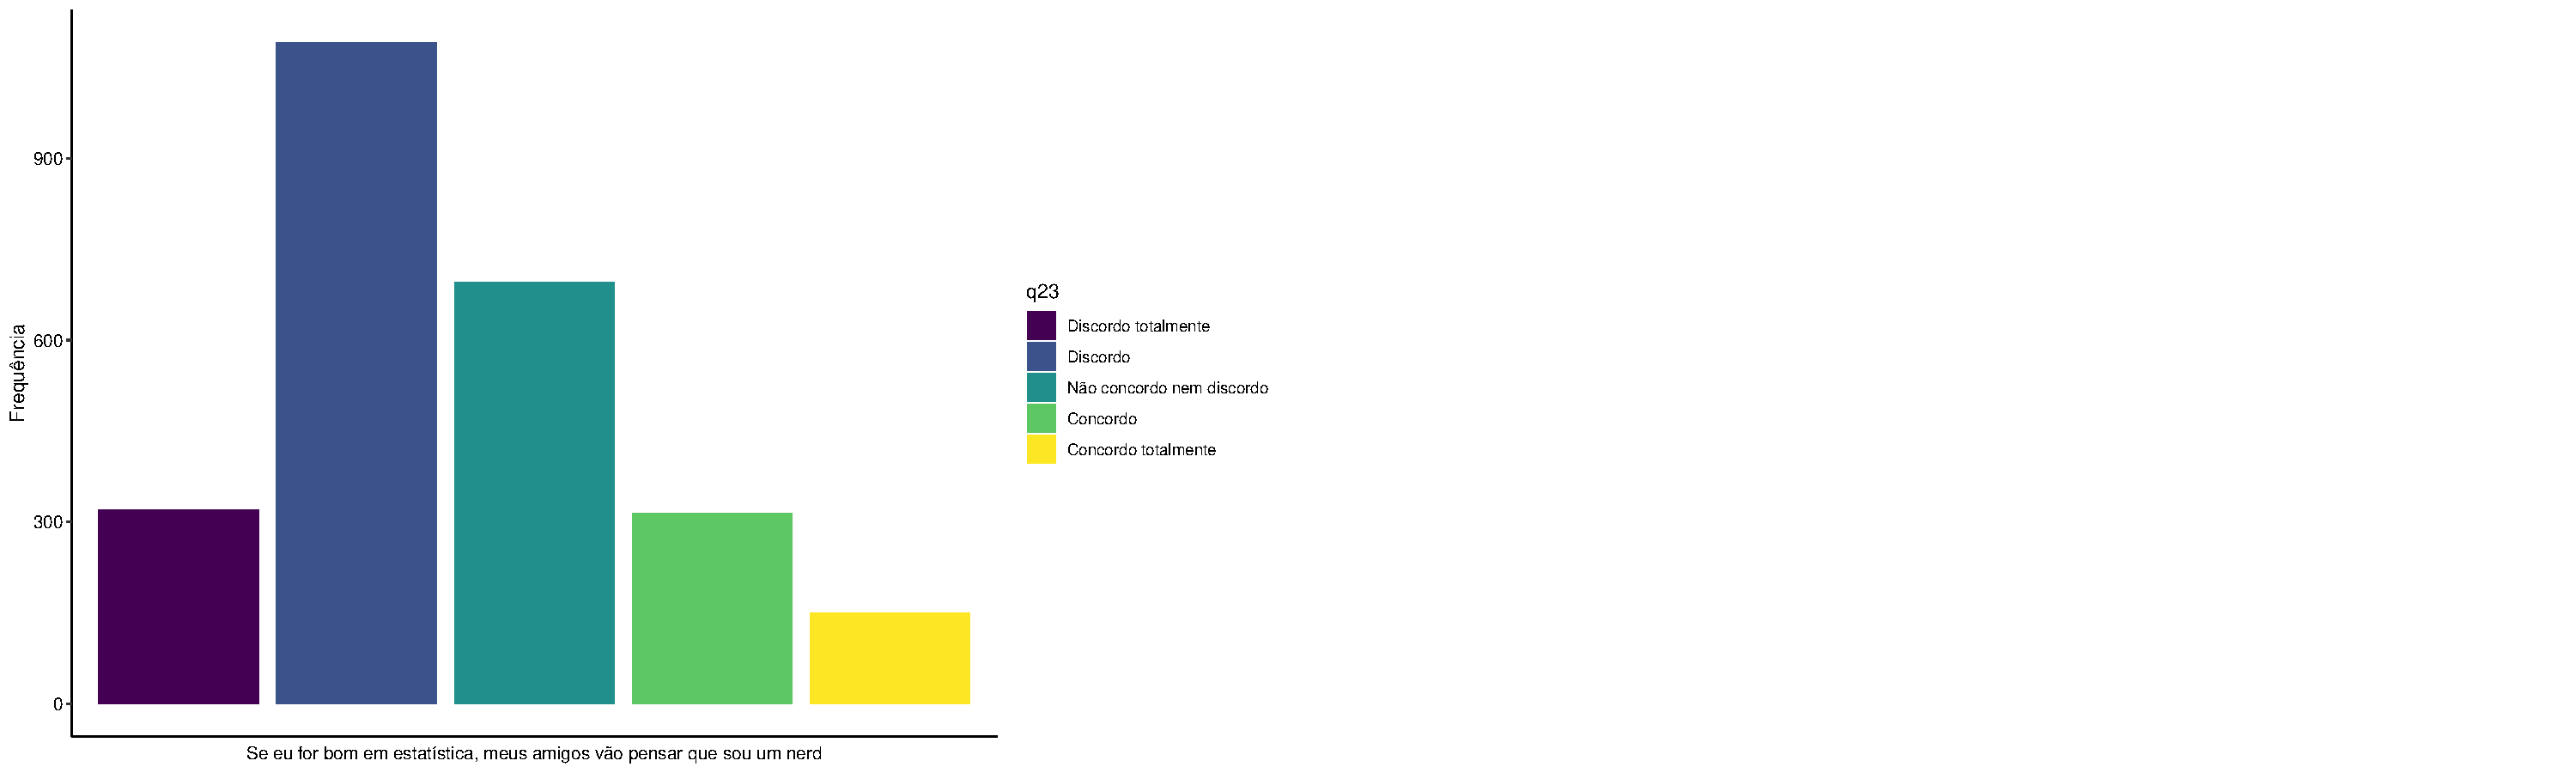
\includegraphics{descritiva_files/figure-pdf/unnamed-chunk-26-12.pdf}

Essa é uma boa forma de olhar os itens, pois temos uma noção geral da
quantidade de cada resposta para cada um deles. Entretanto, caso
quiséssemos medir a ansiedade em relação ao R para cada indivíduo, seria
interessante arranjar uma pontuação para o questionário, representativa
desse construto ansiedade. Para isso, podemos fazer o somatório da
pontuação de cada item, como fizemos na última aula (devemos antes
converter as variáveis para valores numéricos).

\begin{Shaded}
\begin{Highlighting}[]
\CommentTok{\# Cria nova coluna representando pontuação para o questionário}
\NormalTok{factor\_saq }\OtherTok{\textless{}{-}}\NormalTok{ factor\_saq }\SpecialCharTok{|\textgreater{}} 
  \FunctionTok{mutate}\NormalTok{(}\FunctionTok{across}\NormalTok{(q01}\SpecialCharTok{:}\NormalTok{q23, as.numeric)) }\SpecialCharTok{|\textgreater{}} 
  \FunctionTok{rowwise}\NormalTok{() }\SpecialCharTok{|\textgreater{}} 
  \FunctionTok{mutate}\NormalTok{(}\AttributeTok{ansiedade\_r =} \FunctionTok{sum}\NormalTok{(}\FunctionTok{c}\NormalTok{(q01,q02,q03,q04,q05,q07,q07,q08,q09,q10,q11,q12,q13,q14,q15,q16,q17,q18,q19,q20,q21,q22,q23)))}
\end{Highlighting}
\end{Shaded}

Com a nova coluna, podemos agora ver as estatísticas descritivas e fazer
um gráfico de densidade, o nosso somatório representa uma variável
numérica.

\begin{Shaded}
\begin{Highlighting}[]
\CommentTok{\# Estatísticas descritivas para a pontuação do questionário}
\NormalTok{factor\_saq }\SpecialCharTok{|\textgreater{}} 
  \FunctionTok{group\_by}\NormalTok{() }\SpecialCharTok{|\textgreater{}} 
\NormalTok{  dplyr}\SpecialCharTok{::}\FunctionTok{summarise}\NormalTok{(}\AttributeTok{media =} \FunctionTok{mean}\NormalTok{(ansiedade\_r), }\AttributeTok{desvio\_padrao =} \FunctionTok{sd}\NormalTok{(ansiedade\_r), maior\_pontuação }\OtherTok{=} \FunctionTok{max}\NormalTok{(ansiedade\_r), menor\_pontuação }\OtherTok{=} \FunctionTok{min}\NormalTok{(ansiedade\_r), }\AttributeTok{distancia\_interquartil =} \FunctionTok{IQR}\NormalTok{(ansiedade\_r)) }\SpecialCharTok{|\textgreater{}} 
\NormalTok{  knitr}\SpecialCharTok{::}\FunctionTok{kable}\NormalTok{()}
\end{Highlighting}
\end{Shaded}

\begin{longtable}[]{@{}
  >{\raggedleft\arraybackslash}p{(\columnwidth - 8\tabcolsep) * \real{0.1039}}
  >{\raggedleft\arraybackslash}p{(\columnwidth - 8\tabcolsep) * \real{0.1818}}
  >{\raggedleft\arraybackslash}p{(\columnwidth - 8\tabcolsep) * \real{0.2078}}
  >{\raggedleft\arraybackslash}p{(\columnwidth - 8\tabcolsep) * \real{0.2078}}
  >{\raggedleft\arraybackslash}p{(\columnwidth - 8\tabcolsep) * \real{0.2987}}@{}}
\toprule\noalign{}
\begin{minipage}[b]{\linewidth}\raggedleft
media
\end{minipage} & \begin{minipage}[b]{\linewidth}\raggedleft
desvio\_padrao
\end{minipage} & \begin{minipage}[b]{\linewidth}\raggedleft
maior\_pontuação
\end{minipage} & \begin{minipage}[b]{\linewidth}\raggedleft
menor\_pontuação
\end{minipage} & \begin{minipage}[b]{\linewidth}\raggedleft
distancia\_interquartil
\end{minipage} \\
\midrule\noalign{}
\endhead
\bottomrule\noalign{}
\endlastfoot
75.8662 & 9.151513 & 105 & 34 & 12 \\
\end{longtable}

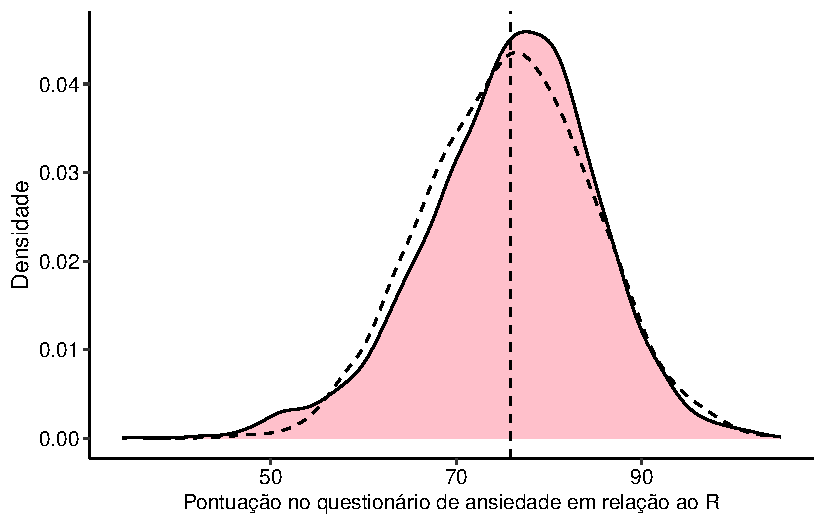
\includegraphics{descritiva_files/figure-pdf/unnamed-chunk-29-1.pdf}

A linnha pontilhada representa uma distribuição normal com mesma média e
desvio padrão. A sobreposição mostra que a distribuição dos somatórios
da pontuação dos itens assemelha-se a uma distribuição normal.

Nesse capítulo vimos um pouco sobre estatística descritiva. Alguns
tópicos não foram abordados, mas espero que tenham conseguido ter uma
noção geral sobre o tema. Na próxima aula, veremos sobre visualização de
dados e estatística inferencial.



\end{document}
